\hypertarget{cha:scales}{%
\chapter{Scales, axes and legends}\label{cha:scales}}

\hypertarget{introduction}{%
\section{Introduction}\label{introduction}}

Scales control the mapping from data to aesthetics. They take your data
and turn it into something that you can see, like size, colour, position
or shape. Scales also provide the tools that let you read the plot: the
axes and legends. Formally, each scale is a function from a region in
data space (the domain of the scale) to a region in aesthetic space (the
range of the scale). The axis or legend is the inverse function: it
allows you to convert visual properties back to data. \index{Scales}

You can generate many plots without knowing how scales work, but
understanding scales and learning how to manipulate them will give you
much more control. The basics of working with scales is described in
\protect\hyperlink{sec:scale-usage}{scale usage}.
\protect\hyperlink{sec:guides}{Guides} discusses the common parameters
that control the axes and legends. Legends are particularly complicated
so have an additional set of options as described in
\protect\hyperlink{sec:legends}{legends}.
\protect\hyperlink{sec:limits}{Limits} shows how to use limits to both
zoom into interesting parts of a plot, and to ensure that multiple plots
have matching legends and axes.
\protect\hyperlink{sec:scale-details}{Scale details} gives an overview
of the different types of scales available in ggplot2, which can be
roughly divided into four categories: continuous position scales, colour
scales, manual scales and identity scales.

\hypertarget{sec:scale-usage}{%
\section{Modifying scales}\label{sec:scale-usage}}

A scale is required for every aesthetic used on the plot. When you
write:

\begin{Shaded}
\begin{Highlighting}[]
\KeywordTok{ggplot}\NormalTok{(mpg, }\KeywordTok{aes}\NormalTok{(displ, hwy)) }\OperatorTok{+}\StringTok{ }
\StringTok{  }\KeywordTok{geom_point}\NormalTok{(}\KeywordTok{aes}\NormalTok{(}\DataTypeTok{colour =}\NormalTok{ class))}
\end{Highlighting}
\end{Shaded}

What actually happens is this:

\begin{Shaded}
\begin{Highlighting}[]
\KeywordTok{ggplot}\NormalTok{(mpg, }\KeywordTok{aes}\NormalTok{(displ, hwy)) }\OperatorTok{+}\StringTok{ }
\StringTok{  }\KeywordTok{geom_point}\NormalTok{(}\KeywordTok{aes}\NormalTok{(}\DataTypeTok{colour =}\NormalTok{ class)) }\OperatorTok{+}
\StringTok{  }\KeywordTok{scale_x_continuous}\NormalTok{() }\OperatorTok{+}\StringTok{ }
\StringTok{  }\KeywordTok{scale_y_continuous}\NormalTok{() }\OperatorTok{+}\StringTok{ }
\StringTok{  }\KeywordTok{scale_colour_discrete}\NormalTok{()}
\end{Highlighting}
\end{Shaded}

Default scales are named according to the aesthetic and the variable
type: \texttt{scale\_y\_continuous()},
\texttt{scale\_colour\_discrete()}, etc.

It would be tedious to manually add a scale every time you used a new
aesthetic, so ggplot2 does it for you. But if you want to override the
defaults, you'll need to add the scale yourself, like this:
\index{Scales!defaults}

\begin{Shaded}
\begin{Highlighting}[]
\KeywordTok{ggplot}\NormalTok{(mpg, }\KeywordTok{aes}\NormalTok{(displ, hwy)) }\OperatorTok{+}\StringTok{ }
\StringTok{  }\KeywordTok{geom_point}\NormalTok{(}\KeywordTok{aes}\NormalTok{(}\DataTypeTok{colour =}\NormalTok{ class)) }\OperatorTok{+}\StringTok{ }
\StringTok{  }\KeywordTok{scale_x_continuous}\NormalTok{(}\StringTok{"A really awesome x axis label"}\NormalTok{) }\OperatorTok{+}
\StringTok{  }\KeywordTok{scale_y_continuous}\NormalTok{(}\StringTok{"An amazingly great y axis label"}\NormalTok{)}
\end{Highlighting}
\end{Shaded}

The use of \texttt{+} to ``add'' scales to a plot is a little
misleading. When you \texttt{+} a scale, you're not actually adding it
to the plot, but overriding the existing scale. This means that the
following two specifications are equivalent: \indexc{+}

\begin{Shaded}
\begin{Highlighting}[]
\KeywordTok{ggplot}\NormalTok{(mpg, }\KeywordTok{aes}\NormalTok{(displ, hwy)) }\OperatorTok{+}\StringTok{ }
\StringTok{  }\KeywordTok{geom_point}\NormalTok{() }\OperatorTok{+}\StringTok{ }
\StringTok{  }\KeywordTok{scale_x_continuous}\NormalTok{(}\StringTok{"Label 1"}\NormalTok{) }\OperatorTok{+}
\StringTok{  }\KeywordTok{scale_x_continuous}\NormalTok{(}\StringTok{"Label 2"}\NormalTok{)}
\CommentTok{#> Scale for 'x' is already present. Adding another scale for 'x',}
\CommentTok{#> which will replace the existing scale.}

\KeywordTok{ggplot}\NormalTok{(mpg, }\KeywordTok{aes}\NormalTok{(displ, hwy)) }\OperatorTok{+}\StringTok{ }
\StringTok{  }\KeywordTok{geom_point}\NormalTok{() }\OperatorTok{+}\StringTok{ }
\StringTok{  }\KeywordTok{scale_x_continuous}\NormalTok{(}\StringTok{"Label 2"}\NormalTok{)}
\end{Highlighting}
\end{Shaded}

Note the message: if you see this in your own code, you need to
reorganise your code specification to only add a single scale.

You can also use a different scale altogether:

\begin{Shaded}
\begin{Highlighting}[]
\KeywordTok{ggplot}\NormalTok{(mpg, }\KeywordTok{aes}\NormalTok{(displ, hwy)) }\OperatorTok{+}\StringTok{ }
\StringTok{  }\KeywordTok{geom_point}\NormalTok{(}\KeywordTok{aes}\NormalTok{(}\DataTypeTok{colour =}\NormalTok{ class)) }\OperatorTok{+}
\StringTok{  }\KeywordTok{scale_x_sqrt}\NormalTok{() }\OperatorTok{+}\StringTok{ }
\StringTok{  }\KeywordTok{scale_colour_brewer}\NormalTok{()}
\end{Highlighting}
\end{Shaded}

You've probably already figured out the naming scheme for scales, but to
be concrete, it's made up of three pieces separated by "\_":
\index{Scales!naming scheme}

\begin{enumerate}
\def\labelenumi{\arabic{enumi}.}
\tightlist
\item
  \texttt{scale}
\item
  The name of the aesthetic (e.g., \texttt{colour}, \texttt{shape} or
  \texttt{x})
\item
  The name of the scale (e.g., \texttt{continuous}, \texttt{discrete},
  \texttt{brewer}).
\end{enumerate}

\hypertarget{exercises}{%
\subsection{Exercises}\label{exercises}}

\begin{enumerate}
\def\labelenumi{\arabic{enumi}.}
\item
  What happens if you pair a discrete variable to a continuous scale?
  What happens if you pair a continuous variable to a discrete scale?
\item
  Simplify the following plot specifications to make them easier to
  understand.

\begin{Shaded}
\begin{Highlighting}[]
\KeywordTok{ggplot}\NormalTok{(mpg, }\KeywordTok{aes}\NormalTok{(displ)) }\OperatorTok{+}\StringTok{ }
\StringTok{  }\KeywordTok{scale_y_continuous}\NormalTok{(}\StringTok{"Highway mpg"}\NormalTok{) }\OperatorTok{+}\StringTok{ }
\StringTok{  }\KeywordTok{scale_x_continuous}\NormalTok{() }\OperatorTok{+}
\StringTok{  }\KeywordTok{geom_point}\NormalTok{(}\KeywordTok{aes}\NormalTok{(}\DataTypeTok{y =}\NormalTok{ hwy))}

\KeywordTok{ggplot}\NormalTok{(mpg, }\KeywordTok{aes}\NormalTok{(}\DataTypeTok{y =}\NormalTok{ displ, }\DataTypeTok{x =}\NormalTok{ class)) }\OperatorTok{+}\StringTok{ }
\StringTok{  }\KeywordTok{scale_y_continuous}\NormalTok{(}\StringTok{"Displacement (l)"}\NormalTok{) }\OperatorTok{+}\StringTok{ }
\StringTok{  }\KeywordTok{scale_x_discrete}\NormalTok{(}\StringTok{"Car type"}\NormalTok{) }\OperatorTok{+}
\StringTok{  }\KeywordTok{scale_x_discrete}\NormalTok{(}\StringTok{"Type of car"}\NormalTok{) }\OperatorTok{+}\StringTok{ }
\StringTok{  }\KeywordTok{scale_colour_discrete}\NormalTok{() }\OperatorTok{+}\StringTok{ }
\StringTok{  }\KeywordTok{geom_point}\NormalTok{(}\KeywordTok{aes}\NormalTok{(}\DataTypeTok{colour =}\NormalTok{ drv)) }\OperatorTok{+}\StringTok{ }
\StringTok{  }\KeywordTok{scale_colour_discrete}\NormalTok{(}\StringTok{"Drive}\CharTok{\textbackslash{}n}\StringTok{train"}\NormalTok{)}
\end{Highlighting}
\end{Shaded}
\end{enumerate}

\hypertarget{sec:guides}{%
\section{Guides: legends and axes}\label{sec:guides}}

The component of a scale that you're most likely to want to modify is
the \textbf{guide}, the axis or legend associated with the scale. Guides
allow you to read observations from the plot and map them back to their
original values. In ggplot2, guides are produced automatically based on
the layers in your plot. This is very different to base R graphics,
where you are responsible for drawing the legends by hand. In ggplot2,
you don't directly control the legend; instead you set up the data so
that there's a clear mapping between data and aesthetics, and a legend
is generated for you automatically. This can be frustrating when you
first start using ggplot2, but once you get the hang of it, you'll find
that it saves you time, and there is little you cannot do. If you're
struggling to get the legend you want, it's likely that your data is in
the wrong form. Read \protect\hyperlink{cha:data}{tidying} to find out
the right form.

You might find it surprising that axes and legends are the same type of
thing, but while they look very different there are many natural
correspondences between the two, as shown in table below and in Figure
\ref{fig:guides}. \index{Guides} \index{Legend} \index{Axis}

\begin{figure}[htbp]
  \centering
  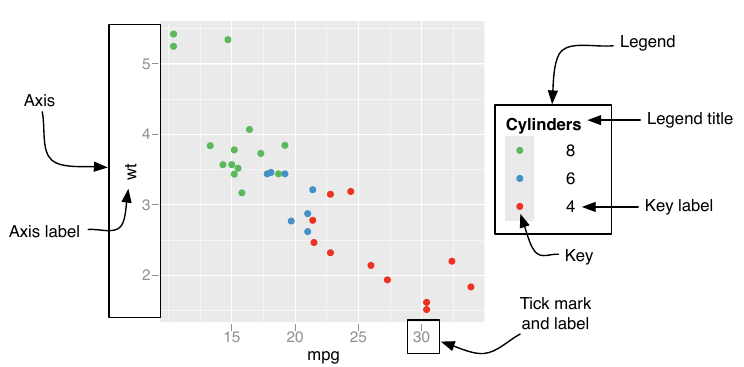
\includegraphics[width=\linewidth]{diagrams/scale-guides.pdf}
  \caption{Axis and legend components}
  \label{fig:guides}
\end{figure}

\begin{longtable}[]{@{}lll@{}}
\toprule
Axis & Legend & Argument name\tabularnewline
\midrule
\endhead
Label & Title & \texttt{name}\tabularnewline
Ticks \& grid line & Key & \texttt{breaks}\tabularnewline
Tick label & Key label & \texttt{labels}\tabularnewline
\bottomrule
\end{longtable}

The following sections covers each of the \texttt{name}, \texttt{breaks}
and \texttt{labels} arguments in more detail.

\hypertarget{scale-title}{%
\subsection{Scale title}\label{scale-title}}

The first argument to the scale function, \texttt{name}, is the
axes/legend title. You can supply text strings (using
\texttt{\textbackslash{}n} for line breaks) or mathematical expressions
in \texttt{quote()} (as described in \texttt{?plotmath}):
\index{Axis!title} \index{Legend!title}

\begin{Shaded}
\begin{Highlighting}[]
\NormalTok{df <-}\StringTok{ }\KeywordTok{data.frame}\NormalTok{(}\DataTypeTok{x =} \DecValTok{1}\OperatorTok{:}\DecValTok{2}\NormalTok{, }\DataTypeTok{y =} \DecValTok{1}\NormalTok{, }\DataTypeTok{z =} \StringTok{"a"}\NormalTok{)}
\NormalTok{p <-}\StringTok{ }\KeywordTok{ggplot}\NormalTok{(df, }\KeywordTok{aes}\NormalTok{(x, y)) }\OperatorTok{+}\StringTok{ }\KeywordTok{geom_point}\NormalTok{()}
\NormalTok{p }\OperatorTok{+}\StringTok{ }\KeywordTok{scale_x_continuous}\NormalTok{(}\StringTok{"X axis"}\NormalTok{)}
\NormalTok{p }\OperatorTok{+}\StringTok{ }\KeywordTok{scale_x_continuous}\NormalTok{(}\KeywordTok{quote}\NormalTok{(a }\OperatorTok{+}\StringTok{ }\NormalTok{mathematical }\OperatorTok{^}\StringTok{ }\NormalTok{expression))}
\end{Highlighting}
\end{Shaded}

\begin{figure}[H]
  \includegraphics[width=0.5\linewidth]{_figures/scales/guide-names-1}%
  \includegraphics[width=0.5\linewidth]{_figures/scales/guide-names-2}
\end{figure}

Because tweaking these labels is such a common task, there are three
helpers that save you some typing: \texttt{xlab()}, \texttt{ylab()} and
\texttt{labs()}:

\begin{Shaded}
\begin{Highlighting}[]
\NormalTok{p <-}\StringTok{ }\KeywordTok{ggplot}\NormalTok{(df, }\KeywordTok{aes}\NormalTok{(x, y)) }\OperatorTok{+}\StringTok{ }\KeywordTok{geom_point}\NormalTok{(}\KeywordTok{aes}\NormalTok{(}\DataTypeTok{colour =}\NormalTok{ z))}
\NormalTok{p }\OperatorTok{+}\StringTok{ }
\StringTok{  }\KeywordTok{xlab}\NormalTok{(}\StringTok{"X axis"}\NormalTok{) }\OperatorTok{+}\StringTok{ }
\StringTok{  }\KeywordTok{ylab}\NormalTok{(}\StringTok{"Y axis"}\NormalTok{)}
\NormalTok{p }\OperatorTok{+}\StringTok{ }\KeywordTok{labs}\NormalTok{(}\DataTypeTok{x =} \StringTok{"X axis"}\NormalTok{, }\DataTypeTok{y =} \StringTok{"Y axis"}\NormalTok{, }\DataTypeTok{colour =} \StringTok{"Colour}\CharTok{\textbackslash{}n}\StringTok{legend"}\NormalTok{)}
\end{Highlighting}
\end{Shaded}

\begin{figure}[H]
  \includegraphics[width=0.5\linewidth]{_figures/scales/guide-names-helper-1}%
  \includegraphics[width=0.5\linewidth]{_figures/scales/guide-names-helper-2}
\end{figure}

There are two ways to remove the axis label. Setting it to \texttt{""}
omits the label, but still allocates space; \texttt{NULL} removes the
label and its space. Look closely at the left and bottom borders of the
following two plots. I've drawn a grey rectangle around the plot to make
it easier to see the difference.

\begin{Shaded}
\begin{Highlighting}[]
\NormalTok{p <-}\StringTok{ }\KeywordTok{ggplot}\NormalTok{(df, }\KeywordTok{aes}\NormalTok{(x, y)) }\OperatorTok{+}\StringTok{ }
\StringTok{  }\KeywordTok{geom_point}\NormalTok{() }\OperatorTok{+}\StringTok{ }
\StringTok{  }\KeywordTok{theme}\NormalTok{(}\DataTypeTok{plot.background =} \KeywordTok{element_rect}\NormalTok{(}\DataTypeTok{colour =} \StringTok{"grey50"}\NormalTok{))}
\NormalTok{p }\OperatorTok{+}\StringTok{ }\KeywordTok{labs}\NormalTok{(}\DataTypeTok{x =} \StringTok{""}\NormalTok{,  }\DataTypeTok{y =} \StringTok{""}\NormalTok{)}
\NormalTok{p }\OperatorTok{+}\StringTok{ }\KeywordTok{labs}\NormalTok{(}\DataTypeTok{x =} \OtherTok{NULL}\NormalTok{, }\DataTypeTok{y =} \OtherTok{NULL}\NormalTok{)}
\end{Highlighting}
\end{Shaded}

\begin{figure}[H]
  \includegraphics[width=0.5\linewidth]{_figures/scales/guide-names-remove-1}%
  \includegraphics[width=0.5\linewidth]{_figures/scales/guide-names-remove-2}
\end{figure}

\hypertarget{breaks-and-labels}{%
\subsection{Breaks and labels}\label{breaks-and-labels}}

The \texttt{breaks} argument controls which values appear as tick marks
on axes and keys on legends. Each break has an associated label,
controlled by the \texttt{labels} argument. If you set \texttt{labels},
you must also set \texttt{breaks}; otherwise, if data changes, the
breaks will no longer align with the labels. \index{Axis!ticks}
\index{Axis!breaks} \index{Axis!labels} \index{Legend!keys}

The following code shows some basic examples for both axes and legends.

\begin{Shaded}
\begin{Highlighting}[]
\NormalTok{df <-}\StringTok{ }\KeywordTok{data.frame}\NormalTok{(}\DataTypeTok{x =} \KeywordTok{c}\NormalTok{(}\DecValTok{1}\NormalTok{, }\DecValTok{3}\NormalTok{, }\DecValTok{5}\NormalTok{) }\OperatorTok{*}\StringTok{ }\DecValTok{1000}\NormalTok{, }\DataTypeTok{y =} \DecValTok{1}\NormalTok{)}
\NormalTok{axs <-}\StringTok{ }\KeywordTok{ggplot}\NormalTok{(df, }\KeywordTok{aes}\NormalTok{(x, y)) }\OperatorTok{+}\StringTok{ }
\StringTok{  }\KeywordTok{geom_point}\NormalTok{() }\OperatorTok{+}\StringTok{ }
\StringTok{  }\KeywordTok{labs}\NormalTok{(}\DataTypeTok{x =} \OtherTok{NULL}\NormalTok{, }\DataTypeTok{y =} \OtherTok{NULL}\NormalTok{)}
\NormalTok{axs}
\NormalTok{axs }\OperatorTok{+}\StringTok{ }\KeywordTok{scale_x_continuous}\NormalTok{(}\DataTypeTok{breaks =} \KeywordTok{c}\NormalTok{(}\DecValTok{2000}\NormalTok{, }\DecValTok{4000}\NormalTok{))}
\NormalTok{axs }\OperatorTok{+}\StringTok{ }\KeywordTok{scale_x_continuous}\NormalTok{(}\DataTypeTok{breaks =} \KeywordTok{c}\NormalTok{(}\DecValTok{2000}\NormalTok{, }\DecValTok{4000}\NormalTok{), }\DataTypeTok{labels =} \KeywordTok{c}\NormalTok{(}\StringTok{"2k"}\NormalTok{, }\StringTok{"4k"}\NormalTok{))}
\end{Highlighting}
\end{Shaded}

\begin{figure}[H]
  \includegraphics[width=0.333\linewidth]{_figures/scales/breaks-labels-1}%
  \includegraphics[width=0.333\linewidth]{_figures/scales/breaks-labels-2}%
  \includegraphics[width=0.333\linewidth]{_figures/scales/breaks-labels-3}
\end{figure}

\begin{Shaded}
\begin{Highlighting}[]
\NormalTok{leg <-}\StringTok{ }\KeywordTok{ggplot}\NormalTok{(df, }\KeywordTok{aes}\NormalTok{(y, x, }\DataTypeTok{fill =}\NormalTok{ x)) }\OperatorTok{+}\StringTok{ }
\StringTok{  }\KeywordTok{geom_tile}\NormalTok{() }\OperatorTok{+}\StringTok{ }
\StringTok{  }\KeywordTok{labs}\NormalTok{(}\DataTypeTok{x =} \OtherTok{NULL}\NormalTok{, }\DataTypeTok{y =} \OtherTok{NULL}\NormalTok{)}
\NormalTok{leg}
\NormalTok{leg }\OperatorTok{+}\StringTok{ }\KeywordTok{scale_fill_continuous}\NormalTok{(}\DataTypeTok{breaks =} \KeywordTok{c}\NormalTok{(}\DecValTok{2000}\NormalTok{, }\DecValTok{4000}\NormalTok{))}
\NormalTok{leg }\OperatorTok{+}\StringTok{ }\KeywordTok{scale_fill_continuous}\NormalTok{(}\DataTypeTok{breaks =} \KeywordTok{c}\NormalTok{(}\DecValTok{2000}\NormalTok{, }\DecValTok{4000}\NormalTok{), }\DataTypeTok{labels =} \KeywordTok{c}\NormalTok{(}\StringTok{"2k"}\NormalTok{, }\StringTok{"4k"}\NormalTok{))}
\end{Highlighting}
\end{Shaded}

\begin{figure}[H]
  \includegraphics[width=0.333\linewidth]{_figures/scales/unnamed-chunk-5-1}%
  \includegraphics[width=0.333\linewidth]{_figures/scales/unnamed-chunk-5-2}%
  \includegraphics[width=0.333\linewidth]{_figures/scales/unnamed-chunk-5-3}
\end{figure}

If you want to relabel the breaks in a categorical scale, you can use a
named labels vector:

\begin{Shaded}
\begin{Highlighting}[]
\NormalTok{df2 <-}\StringTok{ }\KeywordTok{data.frame}\NormalTok{(}\DataTypeTok{x =} \DecValTok{1}\OperatorTok{:}\DecValTok{3}\NormalTok{, }\DataTypeTok{y =} \KeywordTok{c}\NormalTok{(}\StringTok{"a"}\NormalTok{, }\StringTok{"b"}\NormalTok{, }\StringTok{"c"}\NormalTok{))}
\KeywordTok{ggplot}\NormalTok{(df2, }\KeywordTok{aes}\NormalTok{(x, y)) }\OperatorTok{+}\StringTok{ }
\StringTok{  }\KeywordTok{geom_point}\NormalTok{()}
\KeywordTok{ggplot}\NormalTok{(df2, }\KeywordTok{aes}\NormalTok{(x, y)) }\OperatorTok{+}\StringTok{ }
\StringTok{  }\KeywordTok{geom_point}\NormalTok{() }\OperatorTok{+}\StringTok{ }
\StringTok{  }\KeywordTok{scale_y_discrete}\NormalTok{(}\DataTypeTok{labels =} \KeywordTok{c}\NormalTok{(}\DataTypeTok{a =} \StringTok{"apple"}\NormalTok{, }\DataTypeTok{b =} \StringTok{"banana"}\NormalTok{, }\DataTypeTok{c =} \StringTok{"carrot"}\NormalTok{))}
\end{Highlighting}
\end{Shaded}

\begin{figure}[H]
  \includegraphics[width=0.5\linewidth]{_figures/scales/unnamed-chunk-6-1}%
  \includegraphics[width=0.5\linewidth]{_figures/scales/unnamed-chunk-6-2}
\end{figure}

To suppress breaks (and for axes, grid lines) or labels, set them to
\texttt{NULL}:

\begin{Shaded}
\begin{Highlighting}[]
\NormalTok{axs }\OperatorTok{+}\StringTok{ }\KeywordTok{scale_x_continuous}\NormalTok{(}\DataTypeTok{breaks =} \OtherTok{NULL}\NormalTok{)}
\NormalTok{axs }\OperatorTok{+}\StringTok{ }\KeywordTok{scale_x_continuous}\NormalTok{(}\DataTypeTok{labels =} \OtherTok{NULL}\NormalTok{)}
\end{Highlighting}
\end{Shaded}

\begin{figure}[H]
  \includegraphics[width=0.5\linewidth]{_figures/scales/axs-breaks-hide-1}%
  \includegraphics[width=0.5\linewidth]{_figures/scales/axs-breaks-hide-2}
\end{figure}

\begin{Shaded}
\begin{Highlighting}[]
\NormalTok{leg }\OperatorTok{+}\StringTok{ }\KeywordTok{scale_fill_continuous}\NormalTok{(}\DataTypeTok{breaks =} \OtherTok{NULL}\NormalTok{)}
\NormalTok{leg }\OperatorTok{+}\StringTok{ }\KeywordTok{scale_fill_continuous}\NormalTok{(}\DataTypeTok{labels =} \OtherTok{NULL}\NormalTok{)}
\end{Highlighting}
\end{Shaded}

\begin{figure}[H]
  \includegraphics[width=0.5\linewidth]{_figures/scales/leg-breaks-hide-1}%
  \includegraphics[width=0.5\linewidth]{_figures/scales/leg-breaks-hide-2}
\end{figure}

Additionally, you can supply a function to \texttt{breaks} or
\texttt{labels}. The \texttt{breaks} function should have one argument,
the limits (a numeric vector of length two), and should return a numeric
vector of breaks. The \texttt{labels} function should accept a numeric
vector of breaks and return a character vector of labels (the same
length as the input). The scales package provides a number of useful
labelling functions:

\begin{itemize}
\item
  \texttt{scales::comma\_format()} adds commas to make it easier to read
  large numbers.
\item
  \texttt{scales::unit\_format(unit,\ scale)} adds a unit suffix,
  optionally scaling.
\item
  \texttt{scales::dollar\_format(prefix,\ suffix)} displays currency
  values, rounding to two decimal places and adding a prefix or suffix.
\item
  \texttt{scales::wrap\_format()} wraps long labels into multiple lines.
\end{itemize}

See the documentation of the scales package for more details.

\begin{Shaded}
\begin{Highlighting}[]
\NormalTok{axs }\OperatorTok{+}\StringTok{ }\KeywordTok{scale_y_continuous}\NormalTok{(}\DataTypeTok{labels =}\NormalTok{ scales}\OperatorTok{::}\KeywordTok{percent_format}\NormalTok{())}
\NormalTok{axs }\OperatorTok{+}\StringTok{ }\KeywordTok{scale_y_continuous}\NormalTok{(}\DataTypeTok{labels =}\NormalTok{ scales}\OperatorTok{::}\KeywordTok{dollar_format}\NormalTok{(}\DataTypeTok{prefix =} \StringTok{"$"}\NormalTok{))}
\NormalTok{leg }\OperatorTok{+}\StringTok{ }\KeywordTok{scale_fill_continuous}\NormalTok{(}\DataTypeTok{labels =}\NormalTok{ scales}\OperatorTok{::}\KeywordTok{unit_format}\NormalTok{(}\DataTypeTok{unit =} \StringTok{"k"}\NormalTok{, }\DataTypeTok{scale =} \FloatTok{1e-3}\NormalTok{))}
\end{Highlighting}
\end{Shaded}

\begin{figure}[H]
  \includegraphics[width=0.333\linewidth]{_figures/scales/breaks-functions-1}%
  \includegraphics[width=0.333\linewidth]{_figures/scales/breaks-functions-2}%
  \includegraphics[width=0.333\linewidth]{_figures/scales/breaks-functions-3}
\end{figure}

You can adjust the minor breaks (the faint grid lines that appear
between the major grid lines) by supplying a numeric vector of positions
to the \texttt{minor\_breaks} argument. This is particularly useful for
log scales: \index{Minor breaks}

\begin{Shaded}
\begin{Highlighting}[]
\NormalTok{df <-}\StringTok{ }\KeywordTok{data.frame}\NormalTok{(}\DataTypeTok{x =} \KeywordTok{c}\NormalTok{(}\DecValTok{2}\NormalTok{, }\DecValTok{3}\NormalTok{, }\DecValTok{5}\NormalTok{, }\DecValTok{10}\NormalTok{, }\DecValTok{200}\NormalTok{, }\DecValTok{3000}\NormalTok{), }\DataTypeTok{y =} \DecValTok{1}\NormalTok{)}
\KeywordTok{ggplot}\NormalTok{(df, }\KeywordTok{aes}\NormalTok{(x, y)) }\OperatorTok{+}\StringTok{ }
\StringTok{  }\KeywordTok{geom_point}\NormalTok{() }\OperatorTok{+}\StringTok{ }
\StringTok{  }\KeywordTok{scale_x_log10}\NormalTok{()}

\NormalTok{mb <-}\StringTok{ }\KeywordTok{as.numeric}\NormalTok{(}\DecValTok{1}\OperatorTok{:}\DecValTok{10} \OperatorTok\StringTok{ }\DecValTok{10} \OperatorTok{^}\StringTok{ }\NormalTok{(}\DecValTok{0}\OperatorTok{:}\DecValTok{4}\NormalTok{))}
\KeywordTok{ggplot}\NormalTok{(df, }\KeywordTok{aes}\NormalTok{(x, y)) }\OperatorTok{+}\StringTok{ }
\StringTok{  }\KeywordTok{geom_point}\NormalTok{() }\OperatorTok{+}\StringTok{ }
\StringTok{  }\KeywordTok{scale_x_log10}\NormalTok{(}\DataTypeTok{minor_breaks =} \KeywordTok{log10}\NormalTok{(mb))}
\end{Highlighting}
\end{Shaded}

\begin{figure}[H]
  \includegraphics[width=0.5\linewidth]{_figures/scales/unnamed-chunk-7-1}%
  \includegraphics[width=0.5\linewidth]{_figures/scales/unnamed-chunk-7-2}
\end{figure}

Note the use of \texttt{\%o\%} to quickly generate the multiplication
table, and that the minor breaks must be supplied on the transformed
scale. \index{Log!ticks}

\hypertarget{exercises-1}{%
\subsection{Exercises}\label{exercises-1}}

\begin{enumerate}
\def\labelenumi{\arabic{enumi}.}
\item
  Recreate the following graphic:

  \begin{figure}[H]
    \includegraphics[width=0.5\linewidth]{_figures/scales/unnamed-chunk-8-1}
  \end{figure}

  Adjust the y axis label so that the parentheses are the right size.
\item
  List the three different types of object you can supply to the
  \texttt{breaks} argument. How do \texttt{breaks} and \texttt{labels}
  differ?
\item
  Recreate the following plot:

  \begin{figure}[H]
    \includegraphics[width=0.5\linewidth]{_figures/scales/unnamed-chunk-9-1}
  \end{figure}
\item
  What label function allows you to create mathematical expressions?
  What label function converts 1 to 1st, 2 to 2nd, and so on?
\item
  What are the three most important arguments that apply to both axes
  and legends? What do they do? Compare and contrast their operation for
  axes vs.~legends.
\end{enumerate}

\hypertarget{sec:legends}{%
\section{Legends}\label{sec:legends}}

While the most important parameters are shared between axes and legends,
there are some extra options that only apply to legends. Legends are
more complicated than axes because: \index{Legend}

\begin{enumerate}
\def\labelenumi{\arabic{enumi}.}
\item
  A legend can display multiple aesthetics (e.g.~colour and shape), from
  multiple layers, and the symbol displayed in a legend varies based on
  the geom used in the layer.
\item
  Axes always appear in the same place. Legends can appear in different
  places, so you need some global way of controlling them.
\item
  Legends have considerably more details that can be tweaked: should
  they be displayed vertically or horizontally? How many columns? How
  big should the keys be?
\end{enumerate}

The following sections describe the options that control these
interactions.

\hypertarget{sub-layers-legends}{%
\subsection{Layers and legends}\label{sub-layers-legends}}

A legend may need to draw symbols from multiple layers. For example, if
you've mapped colour to both points and lines, the keys will show both
points and lines. If you've mapped fill colour, you get a rectangle.
Note the way the legend varies in the plots below:

\begin{figure}[H]
  \includegraphics[width=0.333\linewidth]{_figures/scales/legend-geom-1}%
  \includegraphics[width=0.333\linewidth]{_figures/scales/legend-geom-2}%
  \includegraphics[width=0.333\linewidth]{_figures/scales/legend-geom-3}
\end{figure}

By default, a layer will only appear if the corresponding aesthetic is
mapped to a variable with \texttt{aes()}. You can override whether or
not a layer appears in the legend with \texttt{show.legend}:
\texttt{FALSE} to prevent a layer from ever appearing in the legend;
\texttt{TRUE} forces it to appear when it otherwise wouldn't. Using
\texttt{TRUE} can be useful in conjunction with the following trick to
make points stand out:

\begin{Shaded}
\begin{Highlighting}[]
\KeywordTok{ggplot}\NormalTok{(df, }\KeywordTok{aes}\NormalTok{(y, y)) }\OperatorTok{+}\StringTok{ }
\StringTok{  }\KeywordTok{geom_point}\NormalTok{(}\DataTypeTok{size =} \DecValTok{4}\NormalTok{, }\DataTypeTok{colour =} \StringTok{"grey20"}\NormalTok{) }\OperatorTok{+}
\StringTok{  }\KeywordTok{geom_point}\NormalTok{(}\KeywordTok{aes}\NormalTok{(}\DataTypeTok{colour =}\NormalTok{ z), }\DataTypeTok{size =} \DecValTok{2}\NormalTok{) }
\KeywordTok{ggplot}\NormalTok{(df, }\KeywordTok{aes}\NormalTok{(y, y)) }\OperatorTok{+}\StringTok{ }
\StringTok{  }\KeywordTok{geom_point}\NormalTok{(}\DataTypeTok{size =} \DecValTok{4}\NormalTok{, }\DataTypeTok{colour =} \StringTok{"grey20"}\NormalTok{, }\DataTypeTok{show.legend =} \OtherTok{TRUE}\NormalTok{) }\OperatorTok{+}
\StringTok{  }\KeywordTok{geom_point}\NormalTok{(}\KeywordTok{aes}\NormalTok{(}\DataTypeTok{colour =}\NormalTok{ z), }\DataTypeTok{size =} \DecValTok{2}\NormalTok{) }
\end{Highlighting}
\end{Shaded}

\begin{figure}[H]
  \includegraphics[width=0.5\linewidth]{_figures/scales/unnamed-chunk-10-1}%
  \includegraphics[width=0.5\linewidth]{_figures/scales/unnamed-chunk-10-2}
\end{figure}

Sometimes you want the geoms in the legend to display differently to the
geoms in the plot. This is particularly useful when you've used
transparency or size to deal with moderate overplotting and also used
colour in the plot. You can do this using the \texttt{override.aes}
parameter of \texttt{guide\_legend()}, which you'll learn more about
shortly. \indexf{override.aes}

\begin{Shaded}
\begin{Highlighting}[]
\NormalTok{norm <-}\StringTok{ }\KeywordTok{data.frame}\NormalTok{(}\DataTypeTok{x =} \KeywordTok{rnorm}\NormalTok{(}\DecValTok{1000}\NormalTok{), }\DataTypeTok{y =} \KeywordTok{rnorm}\NormalTok{(}\DecValTok{1000}\NormalTok{))}
\NormalTok{norm}\OperatorTok{$}\NormalTok{z <-}\StringTok{ }\KeywordTok{cut}\NormalTok{(norm}\OperatorTok{$}\NormalTok{x, }\DecValTok{3}\NormalTok{, }\DataTypeTok{labels =} \KeywordTok{c}\NormalTok{(}\StringTok{"a"}\NormalTok{, }\StringTok{"b"}\NormalTok{, }\StringTok{"c"}\NormalTok{))}
\KeywordTok{ggplot}\NormalTok{(norm, }\KeywordTok{aes}\NormalTok{(x, y)) }\OperatorTok{+}\StringTok{ }
\StringTok{  }\KeywordTok{geom_point}\NormalTok{(}\KeywordTok{aes}\NormalTok{(}\DataTypeTok{colour =}\NormalTok{ z), }\DataTypeTok{alpha =} \FloatTok{0.1}\NormalTok{)}
\KeywordTok{ggplot}\NormalTok{(norm, }\KeywordTok{aes}\NormalTok{(x, y)) }\OperatorTok{+}\StringTok{ }
\StringTok{  }\KeywordTok{geom_point}\NormalTok{(}\KeywordTok{aes}\NormalTok{(}\DataTypeTok{colour =}\NormalTok{ z), }\DataTypeTok{alpha =} \FloatTok{0.1}\NormalTok{) }\OperatorTok{+}\StringTok{ }
\StringTok{  }\KeywordTok{guides}\NormalTok{(}\DataTypeTok{colour =} \KeywordTok{guide_legend}\NormalTok{(}\DataTypeTok{override.aes =} \KeywordTok{list}\NormalTok{(}\DataTypeTok{alpha =} \DecValTok{1}\NormalTok{)))}
\end{Highlighting}
\end{Shaded}

\begin{figure}[H]
  \includegraphics[width=0.5\linewidth]{_figures/scales/unnamed-chunk-11-1}%
  \includegraphics[width=0.5\linewidth]{_figures/scales/unnamed-chunk-11-2}
\end{figure}

ggplot2 tries to use the fewest number of legends to accurately convey
the aesthetics used in the plot. It does this by combining legends where
the same variable is mapped to different aesthetics. The figure below
shows how this works for points: if both colour and shape are mapped to
the same variable, then only a single legend is necessary.
\index{Legend!merging}

\begin{Shaded}
\begin{Highlighting}[]
\KeywordTok{ggplot}\NormalTok{(df, }\KeywordTok{aes}\NormalTok{(x, y)) }\OperatorTok{+}\StringTok{ }\KeywordTok{geom_point}\NormalTok{(}\KeywordTok{aes}\NormalTok{(}\DataTypeTok{colour =}\NormalTok{ z))}
\KeywordTok{ggplot}\NormalTok{(df, }\KeywordTok{aes}\NormalTok{(x, y)) }\OperatorTok{+}\StringTok{ }\KeywordTok{geom_point}\NormalTok{(}\KeywordTok{aes}\NormalTok{(}\DataTypeTok{shape =}\NormalTok{ z))}
\KeywordTok{ggplot}\NormalTok{(df, }\KeywordTok{aes}\NormalTok{(x, y)) }\OperatorTok{+}\StringTok{ }\KeywordTok{geom_point}\NormalTok{(}\KeywordTok{aes}\NormalTok{(}\DataTypeTok{shape =}\NormalTok{ z, }\DataTypeTok{colour =}\NormalTok{ z))}
\end{Highlighting}
\end{Shaded}

\begin{figure}[H]
  \includegraphics[width=0.333\linewidth]{_figures/scales/legend-merge-1}%
  \includegraphics[width=0.333\linewidth]{_figures/scales/legend-merge-2}%
  \includegraphics[width=0.333\linewidth]{_figures/scales/legend-merge-3}
\end{figure}

In order for legends to be merged, they must have the same
\texttt{name}. So if you change the name of one of the scales, you'll
need to change it for all of them.

\hypertarget{sub:legend-layout}{%
\subsection{Legend layout}\label{sub:legend-layout}}

A number of settings that affect the overall display of the legends are
controlled through the theme system. You'll learn more about that in
\protect\hyperlink{sec:themes}{themes}, but for now, all you need to
know is that you modify theme settings with the \texttt{theme()}
function. \index{Themes!legend}

The position and justification of legends are controlled by the theme
setting \texttt{legend.position}, which takes values ``right'',
``left'', ``top'', ``bottom'', or ``none'' (no legend).
\index{Legend!layout}

\begin{Shaded}
\begin{Highlighting}[]
\NormalTok{df <-}\StringTok{ }\KeywordTok{data.frame}\NormalTok{(}\DataTypeTok{x =} \DecValTok{1}\OperatorTok{:}\DecValTok{3}\NormalTok{, }\DataTypeTok{y =} \DecValTok{1}\OperatorTok{:}\DecValTok{3}\NormalTok{, }\DataTypeTok{z =} \KeywordTok{c}\NormalTok{(}\StringTok{"a"}\NormalTok{, }\StringTok{"b"}\NormalTok{, }\StringTok{"c"}\NormalTok{))}
\NormalTok{base <-}\StringTok{ }\KeywordTok{ggplot}\NormalTok{(df, }\KeywordTok{aes}\NormalTok{(x, y)) }\OperatorTok{+}\StringTok{ }
\StringTok{  }\KeywordTok{geom_point}\NormalTok{(}\KeywordTok{aes}\NormalTok{(}\DataTypeTok{colour =}\NormalTok{ z), }\DataTypeTok{size =} \DecValTok{3}\NormalTok{) }\OperatorTok{+}\StringTok{ }
\StringTok{  }\KeywordTok{xlab}\NormalTok{(}\OtherTok{NULL}\NormalTok{) }\OperatorTok{+}\StringTok{ }
\StringTok{  }\KeywordTok{ylab}\NormalTok{(}\OtherTok{NULL}\NormalTok{)}

\NormalTok{base }\OperatorTok{+}\StringTok{ }\KeywordTok{theme}\NormalTok{(}\DataTypeTok{legend.position =} \StringTok{"right"}\NormalTok{) }\CommentTok{# the default }
\NormalTok{base }\OperatorTok{+}\StringTok{ }\KeywordTok{theme}\NormalTok{(}\DataTypeTok{legend.position =} \StringTok{"bottom"}\NormalTok{)}
\NormalTok{base }\OperatorTok{+}\StringTok{ }\KeywordTok{theme}\NormalTok{(}\DataTypeTok{legend.position =} \StringTok{"none"}\NormalTok{)}
\end{Highlighting}
\end{Shaded}

\begin{figure}[H]
  \includegraphics[width=0.333\linewidth]{_figures/scales/legend-position-1}%
  \includegraphics[width=0.333\linewidth]{_figures/scales/legend-position-2}%
  \includegraphics[width=0.333\linewidth]{_figures/scales/legend-position-3}
\end{figure}

Switching between left/right and top/bottom modifies how the keys in
each legend are laid out (horizontal or vertically), and how multiple
legends are stacked (horizontal or vertically). If needed, you can
adjust those options independently:

\begin{itemize}
\item
  \texttt{legend.direction}: layout of items in legends (``horizontal''
  or ``vertical'').
\item
  \texttt{legend.box}: arrangement of multiple legends (``horizontal''
  or ``vertical'').
\item
  \texttt{legend.box.just}: justification of each legend within the
  overall bounding box, when there are multiple legends (``top'',
  ``bottom'', ``left'', or ``right'').
\end{itemize}

Alternatively, if there's a lot of blank space in your plot you might
want to place the legend inside the plot. You can do this by setting
\texttt{legend.position} to a numeric vector of length two. The numbers
represent a relative location in the panel area: \texttt{c(0,\ 1)} is
the top-left corner and \texttt{c(1,\ 0)} is the bottom-right corner.
You control which corner of the legend the \texttt{legend.position}
refers to with \texttt{legend.justification}, which is specified in a
similar way. Unfortunately positioning the legend exactly where you want
it requires a lot of trial and error.

\begin{Shaded}
\begin{Highlighting}[]
\NormalTok{base <-}\StringTok{ }\KeywordTok{ggplot}\NormalTok{(df, }\KeywordTok{aes}\NormalTok{(x, y)) }\OperatorTok{+}\StringTok{ }
\StringTok{  }\KeywordTok{geom_point}\NormalTok{(}\KeywordTok{aes}\NormalTok{(}\DataTypeTok{colour =}\NormalTok{ z), }\DataTypeTok{size =} \DecValTok{3}\NormalTok{)}

\NormalTok{base }\OperatorTok{+}\StringTok{ }\KeywordTok{theme}\NormalTok{(}\DataTypeTok{legend.position =} \KeywordTok{c}\NormalTok{(}\DecValTok{0}\NormalTok{, }\DecValTok{1}\NormalTok{), }\DataTypeTok{legend.justification =} \KeywordTok{c}\NormalTok{(}\DecValTok{0}\NormalTok{, }\DecValTok{1}\NormalTok{))}
\NormalTok{base }\OperatorTok{+}\StringTok{ }\KeywordTok{theme}\NormalTok{(}\DataTypeTok{legend.position =} \KeywordTok{c}\NormalTok{(}\FloatTok{0.5}\NormalTok{, }\FloatTok{0.5}\NormalTok{), }\DataTypeTok{legend.justification =} \KeywordTok{c}\NormalTok{(}\FloatTok{0.5}\NormalTok{, }\FloatTok{0.5}\NormalTok{))}
\NormalTok{base }\OperatorTok{+}\StringTok{ }\KeywordTok{theme}\NormalTok{(}\DataTypeTok{legend.position =} \KeywordTok{c}\NormalTok{(}\DecValTok{1}\NormalTok{, }\DecValTok{0}\NormalTok{), }\DataTypeTok{legend.justification =} \KeywordTok{c}\NormalTok{(}\DecValTok{1}\NormalTok{, }\DecValTok{0}\NormalTok{))}
\end{Highlighting}
\end{Shaded}

\begin{figure}[H]
  \includegraphics[width=0.333\linewidth]{_figures/scales/legend-position-man-1}%
  \includegraphics[width=0.333\linewidth]{_figures/scales/legend-position-man-2}%
  \includegraphics[width=0.333\linewidth]{_figures/scales/legend-position-man-3}
\end{figure}

There's also a margin around the legends, which you can suppress with
\texttt{legend.margin\ =\ unit(0,\ "mm")}.

\hypertarget{guide-functions}{%
\subsection{Guide functions}\label{guide-functions}}

The guide functions, \texttt{guide\_colourbar()} and
\texttt{guide\_legend()}, offer additional control over the fine details
of the legend. Legend guides can be used for any aesthetic (discrete or
continuous) while the colour bar guide can only be used with continuous
colour scales.

You can override the default guide using the \texttt{guide} argument of
the corresponding scale function, or more conveniently, the
\texttt{guides()} helper function. \texttt{guides()} works like
\texttt{labs()}: you can override the default guide associated with each
aesthetic.

\begin{Shaded}
\begin{Highlighting}[]
\NormalTok{df <-}\StringTok{ }\KeywordTok{data.frame}\NormalTok{(}\DataTypeTok{x =} \DecValTok{1}\NormalTok{, }\DataTypeTok{y =} \DecValTok{1}\OperatorTok{:}\DecValTok{3}\NormalTok{, }\DataTypeTok{z =} \DecValTok{1}\OperatorTok{:}\DecValTok{3}\NormalTok{)}
\NormalTok{base <-}\StringTok{ }\KeywordTok{ggplot}\NormalTok{(df, }\KeywordTok{aes}\NormalTok{(x, y)) }\OperatorTok{+}\StringTok{ }\KeywordTok{geom_raster}\NormalTok{(}\KeywordTok{aes}\NormalTok{(}\DataTypeTok{fill =}\NormalTok{ z))}
\NormalTok{base }
\NormalTok{base }\OperatorTok{+}\StringTok{ }\KeywordTok{scale_fill_continuous}\NormalTok{(}\DataTypeTok{guide =} \KeywordTok{guide_legend}\NormalTok{())}
\NormalTok{base }\OperatorTok{+}\StringTok{ }\KeywordTok{guides}\NormalTok{(}\DataTypeTok{fill =} \KeywordTok{guide_legend}\NormalTok{())}
\end{Highlighting}
\end{Shaded}

\begin{figure}[H]
  \includegraphics[width=0.333\linewidth]{_figures/scales/unnamed-chunk-12-1}%
  \includegraphics[width=0.333\linewidth]{_figures/scales/unnamed-chunk-12-2}%
  \includegraphics[width=0.333\linewidth]{_figures/scales/unnamed-chunk-12-3}
\end{figure}

Both functions have numerous examples in their documentation help pages
that illustrate all of their arguments. Most of the arguments to the
guide function control the fine level details of the text colour, size,
font etc. You'll learn about those in the themes chapter. Here I'll
focus on the most important arguments.

\hypertarget{guide_legend}{%
\subsubsection{\texorpdfstring{\texttt{guide\_legend()}}{guide\_legend()}}\label{guide_legend}}

The legend guide displays individual keys in a table. The most useful
options are: \index{Legend!guide}

\begin{itemize}
\item
  \texttt{nrow} or \texttt{ncol} which specify the dimensions of the
  table. \texttt{byrow} controls how the table is filled: \texttt{FALSE}
  fills it by column (the default), \texttt{TRUE} fills it by row.

\begin{Shaded}
\begin{Highlighting}[]
\NormalTok{df <-}\StringTok{ }\KeywordTok{data.frame}\NormalTok{(}\DataTypeTok{x =} \DecValTok{1}\NormalTok{, }\DataTypeTok{y =} \DecValTok{1}\OperatorTok{:}\DecValTok{4}\NormalTok{, }\DataTypeTok{z =}\NormalTok{ letters[}\DecValTok{1}\OperatorTok{:}\DecValTok{4}\NormalTok{])}
\CommentTok{# Base plot}
\NormalTok{p <-}\StringTok{ }\KeywordTok{ggplot}\NormalTok{(df, }\KeywordTok{aes}\NormalTok{(x, y)) }\OperatorTok{+}\StringTok{ }\KeywordTok{geom_raster}\NormalTok{(}\KeywordTok{aes}\NormalTok{(}\DataTypeTok{fill =}\NormalTok{ z))}
\NormalTok{p}
\NormalTok{p }\OperatorTok{+}\StringTok{ }\KeywordTok{guides}\NormalTok{(}\DataTypeTok{fill =} \KeywordTok{guide_legend}\NormalTok{(}\DataTypeTok{ncol =} \DecValTok{2}\NormalTok{))}
\NormalTok{p }\OperatorTok{+}\StringTok{ }\KeywordTok{guides}\NormalTok{(}\DataTypeTok{fill =} \KeywordTok{guide_legend}\NormalTok{(}\DataTypeTok{ncol =} \DecValTok{2}\NormalTok{, }\DataTypeTok{byrow =} \OtherTok{TRUE}\NormalTok{))}
\end{Highlighting}
\end{Shaded}

  \begin{figure}[H]
    \includegraphics[width=0.333\linewidth]{_figures/scales/legend-rows-cols-1}%
    \includegraphics[width=0.333\linewidth]{_figures/scales/legend-rows-cols-2}%
    \includegraphics[width=0.333\linewidth]{_figures/scales/legend-rows-cols-3}
  \end{figure}
\item
  \texttt{reverse} reverses the order of the keys. This is particularly
  useful when you have stacked bars because the default stacking and
  legend orders are different:

\begin{Shaded}
\begin{Highlighting}[]
\NormalTok{p <-}\StringTok{ }\KeywordTok{ggplot}\NormalTok{(df, }\KeywordTok{aes}\NormalTok{(}\DecValTok{1}\NormalTok{, y)) }\OperatorTok{+}\StringTok{ }\KeywordTok{geom_bar}\NormalTok{(}\DataTypeTok{stat =} \StringTok{"identity"}\NormalTok{, }\KeywordTok{aes}\NormalTok{(}\DataTypeTok{fill =}\NormalTok{ z))}
\NormalTok{p}
\NormalTok{p }\OperatorTok{+}\StringTok{ }\KeywordTok{guides}\NormalTok{(}\DataTypeTok{fill =} \KeywordTok{guide_legend}\NormalTok{(}\DataTypeTok{reverse =} \OtherTok{TRUE}\NormalTok{))}
\end{Highlighting}
\end{Shaded}

  \begin{figure}[H]
    \includegraphics[width=0.333\linewidth]{_figures/scales/unnamed-chunk-13-1}%
    \includegraphics[width=0.333\linewidth]{_figures/scales/unnamed-chunk-13-2}
  \end{figure}
\item
  \texttt{override.aes}: override some of the aesthetic settings derived
  from each layer. This is useful if you want to make the elements in
  the legend more visually prominent. See discussion in
  \protect\hyperlink{sub-layers-legends}{layers and legends}.
\item
  \texttt{keywidth} and \texttt{keyheight} (along with
  \texttt{default.unit}) allow you to specify the size of the keys.
  These are grid units, e.g. \texttt{unit(1,\ "cm")}.
\end{itemize}

\hypertarget{guide_colourbar}{%
\subsubsection{\texorpdfstring{\texttt{guide\_colourbar}}{guide\_colourbar}}\label{guide_colourbar}}

The colour bar guide is designed for continuous ranges of colors---as
its name implies, it outputs a rectangle over which the color gradient
varies. The most important arguments are: \index{Legend!colour bar}
\index{Colour bar}

\begin{itemize}
\item
  \texttt{barwidth} and \texttt{barheight} (along with
  \texttt{default.unit}) allow you to specify the size of the bar. These
  are grid units, e.g. \texttt{unit(1,\ "cm")}.
\item
  \texttt{nbin} controls the number of slices. You may want to increase
  this from the default value of 20 if you draw a very long bar.
\item
  \texttt{reverse} flips the colour bar to put the lowest values at the
  top.
\end{itemize}

These options are illustrated below:

\begin{Shaded}
\begin{Highlighting}[]
\NormalTok{df <-}\StringTok{ }\KeywordTok{data.frame}\NormalTok{(}\DataTypeTok{x =} \DecValTok{1}\NormalTok{, }\DataTypeTok{y =} \DecValTok{1}\OperatorTok{:}\DecValTok{4}\NormalTok{, }\DataTypeTok{z =} \DecValTok{4}\OperatorTok{:}\DecValTok{1}\NormalTok{)}
\NormalTok{p <-}\StringTok{ }\KeywordTok{ggplot}\NormalTok{(df, }\KeywordTok{aes}\NormalTok{(x, y)) }\OperatorTok{+}\StringTok{ }\KeywordTok{geom_tile}\NormalTok{(}\KeywordTok{aes}\NormalTok{(}\DataTypeTok{fill =}\NormalTok{ z))}

\NormalTok{p}
\NormalTok{p }\OperatorTok{+}\StringTok{ }\KeywordTok{guides}\NormalTok{(}\DataTypeTok{fill =} \KeywordTok{guide_colorbar}\NormalTok{(}\DataTypeTok{reverse =} \OtherTok{TRUE}\NormalTok{))}
\NormalTok{p }\OperatorTok{+}\StringTok{ }\KeywordTok{guides}\NormalTok{(}\DataTypeTok{fill =} \KeywordTok{guide_colorbar}\NormalTok{(}\DataTypeTok{barheight =} \KeywordTok{unit}\NormalTok{(}\DecValTok{4}\NormalTok{, }\StringTok{"cm"}\NormalTok{)))}
\end{Highlighting}
\end{Shaded}

\begin{figure}[H]
  \includegraphics[width=0.333\linewidth]{_figures/scales/unnamed-chunk-14-1}%
  \includegraphics[width=0.333\linewidth]{_figures/scales/unnamed-chunk-14-2}%
  \includegraphics[width=0.333\linewidth]{_figures/scales/unnamed-chunk-14-3}
\end{figure}

\hypertarget{exercises-2}{%
\subsection{Exercises}\label{exercises-2}}

\begin{enumerate}
\def\labelenumi{\arabic{enumi}.}
\item
  How do you make legends appear to the left of the plot?
\item
  What's gone wrong with this plot? How could you fix it?

\begin{Shaded}
\begin{Highlighting}[]
\KeywordTok{ggplot}\NormalTok{(mpg, }\KeywordTok{aes}\NormalTok{(displ, hwy)) }\OperatorTok{+}\StringTok{ }
\StringTok{  }\KeywordTok{geom_point}\NormalTok{(}\KeywordTok{aes}\NormalTok{(}\DataTypeTok{colour =}\NormalTok{ drv, }\DataTypeTok{shape =}\NormalTok{ drv)) }\OperatorTok{+}\StringTok{ }
\StringTok{  }\KeywordTok{scale_colour_discrete}\NormalTok{(}\StringTok{"Drive train"}\NormalTok{)}
\end{Highlighting}
\end{Shaded}

  \begin{figure}[H]
    \centering
    \includegraphics[width=0.65\linewidth]{_figures/scales/unnamed-chunk-15-1}
  \end{figure}
\item
  Can you recreate the code for this plot?

  \begin{figure}[H]
    \centering
    \includegraphics[width=0.65\linewidth]{_figures/scales/unnamed-chunk-16-1}
  \end{figure}
\end{enumerate}

\hypertarget{sec:limits}{%
\section{Limits}\label{sec:limits}}

The limits, or domain, of a scale are usually derived from the range of
the data. \index{Axis!limits} \index{Scales!limits} There are two
reasons you might want to specify limits rather than relying on the
data:

\begin{enumerate}
\def\labelenumi{\arabic{enumi}.}
\item
  You want to make limits smaller than the range of the data to focus on
  an interesting area of the plot.
\item
  You want to make the limits larger than the range of the data because
  you want multiple plots to match up.
\end{enumerate}

It's most natural to think about the limits of position scales: they map
directly to the ranges of the axes. But limits also apply to scales that
have legends, like colour, size, and shape. This is particularly
important to realise if you want your colours to match up across
multiple plots in your paper.

You can modify the limits using the \texttt{limits} parameter of the
scale:

\begin{itemize}
\item
  For continuous scales, this should be a numeric vector of length two.
  If you only want to set the upper or lower limit, you can set the
  other value to \texttt{NA}.
\item
  For discrete scales, this is a character vector which enumerates all
  possible values.
\end{itemize}

\begin{Shaded}
\begin{Highlighting}[]
\NormalTok{df <-}\StringTok{ }\KeywordTok{data.frame}\NormalTok{(}\DataTypeTok{x =} \DecValTok{1}\OperatorTok{:}\DecValTok{3}\NormalTok{, }\DataTypeTok{y =} \DecValTok{1}\OperatorTok{:}\DecValTok{3}\NormalTok{)}
\NormalTok{base <-}\StringTok{ }\KeywordTok{ggplot}\NormalTok{(df, }\KeywordTok{aes}\NormalTok{(x, y)) }\OperatorTok{+}\StringTok{ }\KeywordTok{geom_point}\NormalTok{() }

\NormalTok{base}
\NormalTok{base }\OperatorTok{+}\StringTok{ }\KeywordTok{scale_x_continuous}\NormalTok{(}\DataTypeTok{limits =} \KeywordTok{c}\NormalTok{(}\FloatTok{1.5}\NormalTok{, }\FloatTok{2.5}\NormalTok{))}
\CommentTok{#> Warning: Removed 2 rows containing missing values (geom_point).}
\NormalTok{base }\OperatorTok{+}\StringTok{ }\KeywordTok{scale_x_continuous}\NormalTok{(}\DataTypeTok{limits =} \KeywordTok{c}\NormalTok{(}\DecValTok{0}\NormalTok{, }\DecValTok{4}\NormalTok{))}
\end{Highlighting}
\end{Shaded}

\begin{figure}[H]
  \includegraphics[width=0.333\linewidth]{_figures/scales/unnamed-chunk-17-1}%
  \includegraphics[width=0.333\linewidth]{_figures/scales/unnamed-chunk-17-2}%
  \includegraphics[width=0.333\linewidth]{_figures/scales/unnamed-chunk-17-3}
\end{figure}

Because modifying the limits is such a common task, ggplot2 provides
some helper to make this even easier: \texttt{xlim()}, \texttt{ylim()}
and \texttt{lims()} These functions inspect their input and then create
the appropriate scale, as follows: \indexf{xlim} \indexf{ylim}

\begin{itemize}
\tightlist
\item
  \texttt{xlim(10,\ 20)}: a continuous scale from 10 to 20
\item
  \texttt{ylim(20,\ 10)}: a reversed continuous scale from 20 to 10
\item
  \texttt{xlim("a",\ "b",\ "c")}: a discrete scale
\item
  \texttt{xlim(as.Date(c("2008-05-01",\ "2008-08-01")))}: a date scale
  from May 1 to August 1 2008.
\end{itemize}

\begin{Shaded}
\begin{Highlighting}[]
\NormalTok{base }\OperatorTok{+}\StringTok{ }\KeywordTok{xlim}\NormalTok{(}\DecValTok{0}\NormalTok{, }\DecValTok{4}\NormalTok{)}
\NormalTok{base }\OperatorTok{+}\StringTok{ }\KeywordTok{xlim}\NormalTok{(}\DecValTok{4}\NormalTok{, }\DecValTok{0}\NormalTok{)}
\NormalTok{base }\OperatorTok{+}\StringTok{ }\KeywordTok{lims}\NormalTok{(}\DataTypeTok{x =} \KeywordTok{c}\NormalTok{(}\DecValTok{0}\NormalTok{, }\DecValTok{4}\NormalTok{))}
\end{Highlighting}
\end{Shaded}

\begin{figure}[H]
  \includegraphics[width=0.333\linewidth]{_figures/scales/unnamed-chunk-18-1}%
  \includegraphics[width=0.333\linewidth]{_figures/scales/unnamed-chunk-18-2}%
  \includegraphics[width=0.333\linewidth]{_figures/scales/unnamed-chunk-18-3}
\end{figure}

If you have eagle eyes, you'll have noticed that the range of the axes
actually extends a little bit past the limits that you've specified.
This ensures that the data does not overlap the axes. To eliminate this
space, set \texttt{expand\ =\ c(0,\ 0)}. This is useful in conjunction
with \texttt{geom\_raster()}: \index{Axis!expansion}

\begin{Shaded}
\begin{Highlighting}[]
\KeywordTok{ggplot}\NormalTok{(faithfuld, }\KeywordTok{aes}\NormalTok{(waiting, eruptions)) }\OperatorTok{+}\StringTok{ }
\StringTok{  }\KeywordTok{geom_raster}\NormalTok{(}\KeywordTok{aes}\NormalTok{(}\DataTypeTok{fill =}\NormalTok{ density)) }\OperatorTok{+}\StringTok{ }
\StringTok{  }\KeywordTok{theme}\NormalTok{(}\DataTypeTok{legend.position =} \StringTok{"none"}\NormalTok{)}
\KeywordTok{ggplot}\NormalTok{(faithfuld, }\KeywordTok{aes}\NormalTok{(waiting, eruptions)) }\OperatorTok{+}\StringTok{ }
\StringTok{  }\KeywordTok{geom_raster}\NormalTok{(}\KeywordTok{aes}\NormalTok{(}\DataTypeTok{fill =}\NormalTok{ density)) }\OperatorTok{+}\StringTok{ }
\StringTok{  }\KeywordTok{scale_x_continuous}\NormalTok{(}\DataTypeTok{expand =} \KeywordTok{c}\NormalTok{(}\DecValTok{0}\NormalTok{,}\DecValTok{0}\NormalTok{)) }\OperatorTok{+}\StringTok{ }
\StringTok{  }\KeywordTok{scale_y_continuous}\NormalTok{(}\DataTypeTok{expand =} \KeywordTok{c}\NormalTok{(}\DecValTok{0}\NormalTok{,}\DecValTok{0}\NormalTok{)) }\OperatorTok{+}
\StringTok{  }\KeywordTok{theme}\NormalTok{(}\DataTypeTok{legend.position =} \StringTok{"none"}\NormalTok{)}
\end{Highlighting}
\end{Shaded}

\begin{figure}[H]
  \centering
  \includegraphics[width=0.33\linewidth]{_figures/scales/unnamed-chunk-19-1}%
  \includegraphics[width=0.33\linewidth]{_figures/scales/unnamed-chunk-19-2}
\end{figure}

By default, any data outside the limits is converted to \texttt{NA}.
This means that setting the limits is not the same as visually zooming
in to a region of the plot. To do that, you need to use the
\texttt{xlim} and \texttt{ylim} arguments to
\texttt{coord\_cartesian()}, described in
\protect\hyperlink{sub:cartesian}{cartesian coordinate systems}. This
performs purely visual zooming and does not affect the underlying data.
\index{Zooming} You can override this with the \texttt{oob} (out of
bounds) argument to the scale. The default is \texttt{scales::censor()}
which replaces any value outside the limits with \texttt{NA}. Another
option is \texttt{scales::squish()} which squishes all values into the
range:

\begin{Shaded}
\begin{Highlighting}[]
\NormalTok{df <-}\StringTok{ }\KeywordTok{data.frame}\NormalTok{(}\DataTypeTok{x =} \DecValTok{1}\OperatorTok{:}\DecValTok{5}\NormalTok{)}
\NormalTok{p <-}\StringTok{ }\KeywordTok{ggplot}\NormalTok{(df, }\KeywordTok{aes}\NormalTok{(x, }\DecValTok{1}\NormalTok{)) }\OperatorTok{+}\StringTok{ }\KeywordTok{geom_tile}\NormalTok{(}\KeywordTok{aes}\NormalTok{(}\DataTypeTok{fill =}\NormalTok{ x), }\DataTypeTok{colour =} \StringTok{"white"}\NormalTok{)}
\NormalTok{p}
\NormalTok{p }\OperatorTok{+}\StringTok{ }\KeywordTok{scale_fill_gradient}\NormalTok{(}\DataTypeTok{limits =} \KeywordTok{c}\NormalTok{(}\DecValTok{2}\NormalTok{, }\DecValTok{4}\NormalTok{))}
\NormalTok{p }\OperatorTok{+}\StringTok{ }\KeywordTok{scale_fill_gradient}\NormalTok{(}\DataTypeTok{limits =} \KeywordTok{c}\NormalTok{(}\DecValTok{2}\NormalTok{, }\DecValTok{4}\NormalTok{), }\DataTypeTok{oob =}\NormalTok{ scales}\OperatorTok{::}\NormalTok{squish)}
\end{Highlighting}
\end{Shaded}

\begin{figure}[H]
  \centering
  \includegraphics[width=0.33\linewidth]{_figures/scales/unnamed-chunk-20-1}%
  \includegraphics[width=0.33\linewidth]{_figures/scales/unnamed-chunk-20-2}%
  \includegraphics[width=0.33\linewidth]{_figures/scales/unnamed-chunk-20-3}
\end{figure}

\hypertarget{exercises-3}{%
\subsection{Exercises}\label{exercises-3}}

\begin{enumerate}
\def\labelenumi{\arabic{enumi}.}
\item
  The following code creates two plots of the mpg dataset. Modify the
  code so that the legend and axes match, without using facetting!

\begin{Shaded}
\begin{Highlighting}[]
\NormalTok{fwd <-}\StringTok{ }\KeywordTok{subset}\NormalTok{(mpg, drv }\OperatorTok{==}\StringTok{ "f"}\NormalTok{)}
\NormalTok{rwd <-}\StringTok{ }\KeywordTok{subset}\NormalTok{(mpg, drv }\OperatorTok{==}\StringTok{ "r"}\NormalTok{)}

\KeywordTok{ggplot}\NormalTok{(fwd, }\KeywordTok{aes}\NormalTok{(displ, hwy, }\DataTypeTok{colour =}\NormalTok{ class)) }\OperatorTok{+}\StringTok{ }\KeywordTok{geom_point}\NormalTok{()}
\KeywordTok{ggplot}\NormalTok{(rwd, }\KeywordTok{aes}\NormalTok{(displ, hwy, }\DataTypeTok{colour =}\NormalTok{ class)) }\OperatorTok{+}\StringTok{ }\KeywordTok{geom_point}\NormalTok{()}
\end{Highlighting}
\end{Shaded}

  \begin{figure}[H]
    \includegraphics[width=0.5\linewidth]{_figures/scales/unnamed-chunk-21-1}%
    \includegraphics[width=0.5\linewidth]{_figures/scales/unnamed-chunk-21-2}
  \end{figure}
\item
  What does \texttt{expand\_limits()} do and how does it work? Read the
  source code.
\item
  What happens if you add two \texttt{xlim()} calls to the same plot?
  Why?
\item
  What does \texttt{scale\_x\_continuous(limits\ =\ c(NA,\ NA))} do?
\end{enumerate}

\hypertarget{sec:scale-details}{%
\section{Scales toolbox}\label{sec:scale-details}}

As well as tweaking the options of the default scales, you can also
override them completely with new scales. Scales can be divided roughly
into four families:

\begin{itemize}
\item
  Continuous position scales used to map integer, numeric, and date/time
  data to x and y position.
\item
  Colour scales, used to map continuous and discrete data to colours.
\item
  Manual scales, used to map discrete variables to your choice of size,
  line type, shape or colour.
\item
  The identity scale, paradoxically used to plot variables
  \emph{without} scaling them. This is useful if your data is already a
  vector of colour names.
\end{itemize}

The follow sections describe each family in more detail.

\hypertarget{sub:scale-position}{%
\subsection{Continuous position scales}\label{sub:scale-position}}

Every plot has two position scales, x and y. \index{Scales!position}
\index{Positioning!scales} The most common continuous position scales
are \texttt{scale\_x\_continuous()} and \texttt{scale\_y\_continuous()},
which linearly map data to the x and y axis. \index{Scales!position}
\index{Transformation!scales} \indexf{scale\_x\_continuous} The most
interesting variations are produced using transformations. Every
continuous scale takes a \texttt{trans} argument, allowing the use of a
variety of transformations:

\begin{Shaded}
\begin{Highlighting}[]
\CommentTok{# Convert from fuel economy to fuel consumption}
\KeywordTok{ggplot}\NormalTok{(mpg, }\KeywordTok{aes}\NormalTok{(displ, hwy)) }\OperatorTok{+}\StringTok{ }
\StringTok{  }\KeywordTok{geom_point}\NormalTok{() }\OperatorTok{+}\StringTok{ }
\StringTok{  }\KeywordTok{scale_y_continuous}\NormalTok{(}\DataTypeTok{trans =} \StringTok{"reciprocal"}\NormalTok{)}

\CommentTok{# Log transform x and y axes}
\KeywordTok{ggplot}\NormalTok{(diamonds, }\KeywordTok{aes}\NormalTok{(price, carat)) }\OperatorTok{+}\StringTok{ }
\StringTok{  }\KeywordTok{geom_bin2d}\NormalTok{() }\OperatorTok{+}\StringTok{ }
\StringTok{  }\KeywordTok{scale_x_continuous}\NormalTok{(}\DataTypeTok{trans =} \StringTok{"log10"}\NormalTok{) }\OperatorTok{+}
\StringTok{  }\KeywordTok{scale_y_continuous}\NormalTok{(}\DataTypeTok{trans =} \StringTok{"log10"}\NormalTok{)}
\end{Highlighting}
\end{Shaded}

\begin{figure}[H]
  \includegraphics[width=0.5\linewidth]{_figures/scales/unnamed-chunk-22-1}%
  \includegraphics[width=0.5\linewidth]{_figures/scales/unnamed-chunk-22-2}
\end{figure}

The transformation is carried out by a ``transformer'', which describes
the transformation, its inverse, and how to draw the labels. The
following table lists the most common variants:

\begin{longtable}[]{@{}lll@{}}
\toprule
Name & Function \(f(x)\) & Inverse \(f^{-1}(y)\)\tabularnewline
\midrule
\endhead
asn & \(\tanh^{-1}(x)\) & \(\tanh(y)\)\tabularnewline
exp & \(e ^ x\) & \(\log(y)\)\tabularnewline
identity & \(x\) & \(y\)\tabularnewline
log & \(\log(x)\) & \(e ^ y\)\tabularnewline
log10 & \(\log_{10}(x)\) & \(10 ^ y\)\tabularnewline
log2 & \(\log_2(x)\) & \(2 ^ y\)\tabularnewline
logit & \(\log(\frac{x}{1 - x})\) &
\(\frac{1}{1 + e(y)}\)\tabularnewline
pow10 & \(10^x\) & \(\log_{10}(y)\)\tabularnewline
probit & \(\Phi(x)\) & \(\Phi^{-1}(y)\)\tabularnewline
reciprocal & \(x^{-1}\) & \(y^{-1}\)\tabularnewline
reverse & \(-x\) & \(-y\)\tabularnewline
sqrt & \(x^{1/2}\) & \(y ^ 2\)\tabularnewline
\bottomrule
\end{longtable}

There are shortcuts for the most common: \texttt{scale\_x\_log10()},
\texttt{scale\_x\_sqrt()} and \texttt{scale\_x\_reverse()} (and
similarly for \texttt{y}.) \index{Log!scale} \indexf{scale\_x\_log10}

Of course, you can also perform the transformation yourself. For
example, instead of using \texttt{scale\_x\_log10()}, you could plot
\texttt{log10(x)}. The appearance of the geom will be the same, but the
tick labels will be different. If you use a transformed scale, the axes
will be labelled in the original data space; if you transform the data,
the axes will be labelled in the transformed space.

In either case, the transformation occurs before any statistical
summaries. To transform, \emph{after} statistical computation, use
\texttt{coord\_trans()}. See \protect\hyperlink{sub:cartesian}{cartesian
coordinate systems} for more details.

Date and date/time data are continuous variables with special labels.
ggplot2 works with \texttt{Date} (for dates) and \texttt{POSIXct} (for
date/times) classes: if your dates are in a different format you will
need to convert them with \texttt{as.Date()} or \texttt{as.POSIXct()}.
\index{Date/times} \index{Data!date/time} \index{Time}
\index{Scales!date/time} \indexf{scale\_x\_datetime}
\texttt{scale\_x\_date()} and \texttt{scale\_x\_datetime()} work
similarly to \texttt{scale\_x\_continuous()} but have special
\texttt{date\_breaks} and \texttt{date\_labels} arguments that work in
date-friendly units:

\begin{itemize}
\item
  \texttt{date\_breaks} and \texttt{date\_minor\_breaks()} allows you to
  position breaks by date units (years, months, weeks, days, hours,
  minutes, and seconds). For example,
  \texttt{date\_breaks\ =\ "2\ weeks"} will place a major tick mark
  every two weeks.
\item
  \texttt{date\_labels} controls the display of the labels using the
  same formatting strings as in \texttt{strptime()} and
  \texttt{format()}:

  \begin{longtable}[]{@{}ll@{}}
  \toprule
  String & Meaning\tabularnewline
  \midrule
  \endhead
  \texttt{\%S} & second (00-59)\tabularnewline
  \texttt{\%M} & minute (00-59)\tabularnewline
  \texttt{\%l} & hour, in 12-hour clock (1-12)\tabularnewline
  \texttt{\%I} & hour, in 12-hour clock (01-12)\tabularnewline
  \texttt{\%p} & am/pm\tabularnewline
  \texttt{\%H} & hour, in 24-hour clock (00-23)\tabularnewline
  \texttt{\%a} & day of week, abbreviated (Mon-Sun)\tabularnewline
  \texttt{\%A} & day of week, full (Monday-Sunday)\tabularnewline
  \texttt{\%e} & day of month (1-31)\tabularnewline
  \texttt{\%d} & day of month (01-31)\tabularnewline
  \texttt{\%m} & month, numeric (01-12)\tabularnewline
  \texttt{\%b} & month, abbreviated (Jan-Dec)\tabularnewline
  \texttt{\%B} & month, full (January-December)\tabularnewline
  \texttt{\%y} & year, without century (00-99)\tabularnewline
  \texttt{\%Y} & year, with century (0000-9999)\tabularnewline
  \bottomrule
  \end{longtable}

  For example, if you wanted to display dates like 14/10/1979, you would
  use the string \texttt{"\%d/\%m/\%Y"}.
\end{itemize}

The code below illustrates some of these parameters.

\begin{Shaded}
\begin{Highlighting}[]
\NormalTok{base <-}\StringTok{ }\KeywordTok{ggplot}\NormalTok{(economics, }\KeywordTok{aes}\NormalTok{(date, psavert)) }\OperatorTok{+}\StringTok{ }
\StringTok{  }\KeywordTok{geom_line}\NormalTok{(}\DataTypeTok{na.rm =} \OtherTok{TRUE}\NormalTok{) }\OperatorTok{+}
\StringTok{  }\KeywordTok{labs}\NormalTok{(}\DataTypeTok{x =} \OtherTok{NULL}\NormalTok{, }\DataTypeTok{y =} \OtherTok{NULL}\NormalTok{)}

\NormalTok{base }\CommentTok{# Default breaks and labels}
\NormalTok{base }\OperatorTok{+}\StringTok{ }\KeywordTok{scale_x_date}\NormalTok{(}\DataTypeTok{date_labels =} \StringTok{"%y"}\NormalTok{, }\DataTypeTok{date_breaks =} \StringTok{"5 years"}\NormalTok{)}
\end{Highlighting}
\end{Shaded}

\begin{figure}[H]
  \includegraphics[width=0.5\linewidth]{_figures/scales/date-scale-1}%
  \includegraphics[width=0.5\linewidth]{_figures/scales/date-scale-2}
\end{figure}

\begin{Shaded}
\begin{Highlighting}[]
\NormalTok{base }\OperatorTok{+}\StringTok{ }\KeywordTok{scale_x_date}\NormalTok{(}
  \DataTypeTok{limits =} \KeywordTok{as.Date}\NormalTok{(}\KeywordTok{c}\NormalTok{(}\StringTok{"2004-01-01"}\NormalTok{, }\StringTok{"2005-01-01"}\NormalTok{)),}
  \DataTypeTok{date_labels =} \StringTok{"%b %y"}\NormalTok{,}
  \DataTypeTok{date_minor_breaks =} \StringTok{"1 month"}
\NormalTok{)}
\NormalTok{base }\OperatorTok{+}\StringTok{ }\KeywordTok{scale_x_date}\NormalTok{(}
  \DataTypeTok{limits =} \KeywordTok{as.Date}\NormalTok{(}\KeywordTok{c}\NormalTok{(}\StringTok{"2004-01-01"}\NormalTok{, }\StringTok{"2004-06-01"}\NormalTok{)),}
  \DataTypeTok{date_labels =} \StringTok{"%m/%d"}\NormalTok{,}
  \DataTypeTok{date_minor_breaks =} \StringTok{"2 weeks"}
\NormalTok{)}
\end{Highlighting}
\end{Shaded}

\begin{figure}[H]
  \includegraphics[width=0.5\linewidth]{_figures/scales/date-scale-2-1}%
  \includegraphics[width=0.5\linewidth]{_figures/scales/date-scale-2-2}
\end{figure}

\hypertarget{sub:scale-colour}{%
\subsection{Colour}\label{sub:scale-colour}}

After position, the most commonly used aesthetic is colour. There are
quite a few different ways of mapping values to colours in ggplot2: four
different gradient-based methods for continuous values, and two methods
for mapping discrete values. But before we look at the details of the
different methods, it's useful to learn a little bit of colour theory.
Colour theory is complex because the underlying biology of the eye and
brain is complex, and this introduction will only touch on some of the
more important issues. An excellent and more detailed exposition is
available online at \url{http://tinyurl.com/clrdtls}. \index{Colour}
\index{Scales!colour}

At the physical level, colour is produced by a mixture of wavelengths of
light. To characterise a colour completely, we need to know the complete
mixture of wavelengths. Fortunately for us the human eye only has three
different colour receptors, and so we can summarise the perception of
any colour with just three numbers. You may be familiar with the RGB
encoding of colour space, which defines a colour by the intensities of
red, green and blue light needed to produce it. One problem with this
space is that it is not perceptually uniform: the two colours that are
one unit apart may look similar or very different depending on where
they are in the colour space. This makes it difficult to create a
mapping from a continuous variable to a set of colours. There have been
many attempts to come up with colours spaces that are more perceptually
uniform. We'll use a modern attempt called the HCL colour space, which
has three components of \textbf{h}ue, \textbf{c}hroma and
\textbf{l}uminance: \index{Colour!spaces}

\begin{itemize}
\item
  Hue is a number between 0 and 360 (an angle) which gives the
  ``colour'' of the colour: like blue, red, orange, etc.
\item
  Chroma is the purity of a colour. A chroma of 0 is grey, and the
  maximum value of chroma varies with luminance.
\item
  Luminance is the lightness of the colour. A luminance of 0 produces
  black, and a luminance of 1 produces white.
\end{itemize}

Hues are not perceived as being ordered: e.g.~green does not seem
``larger'' than red. The perception of chroma and luminance are ordered.

The combination of these three components does not produce a simple
geometric shape. Figure \ref{fig:hcl} attempts to show the 3d shape of
the space. Each slice is a constant luminance (brightness) with hue
mapped to angle and chroma to radius. You can see the centre of each
slice is grey and the colours get more intense as they get closer to the
edge.

\begin{figure}[htbp]
  \centering
    \includegraphics[width=\linewidth]{diagrams/hcl-space}
  \caption{The shape of the HCL colour space.  Hue is mapped to angle, chroma to radius and each slice shows a different luminance.  The HCL space is a pretty odd shape, but you can see that colours near the centre of each slice are grey, and as you move towards the edges they become more intense.  Slices for luminance 0 and 100 are omitted because they would, respectively, be a single black point and a single white point.}
  \label{fig:hcl}
\end{figure}

An additional complication is that many people (\textasciitilde{}10\% of
men) do not possess the normal complement of colour receptors and so can
distinguish fewer colours than usual. \index{Colour!blindness} In brief,
it's best to avoid red-green contrasts, and to check your plots with
systems that simulate colour blindness. Visicheck is one online
solution. Another alternative is the \textbf{dichromat} package (Lumley
2007) which provides tools for simulating colour blindness, and a set of
colour schemes known to work well for colour-blind people. You can also
help people with colour blindness in the same way that you can help
people with black-and-white printers: by providing redundant mappings to
other aesthetics like size, line type or shape.

\hypertarget{ssub:colour-continuous}{%
\subsubsection{Continuous}\label{ssub:colour-continuous}}

Colour gradients are often used to show the height of a 2d surface. In
the following example we'll use the surface of a 2d density estimate of
the \texttt{faithful} dataset (Azzalini and Bowman 1990), which records
the waiting time between eruptions and during each eruption for the Old
Faithful geyser in Yellowstone Park. I hide the legends and set
\texttt{expand} to 0, to focus on the appearance of the data.
\index{Colour!gradients} \index{Scales!colour}. Remember: I'm
illustrating these scales with filled tiles, but you can also use them
with coloured lines and points.

\begin{Shaded}
\begin{Highlighting}[]
\NormalTok{erupt <-}\StringTok{ }\KeywordTok{ggplot}\NormalTok{(faithfuld, }\KeywordTok{aes}\NormalTok{(waiting, eruptions, }\DataTypeTok{fill =}\NormalTok{ density)) }\OperatorTok{+}
\StringTok{  }\KeywordTok{geom_raster}\NormalTok{() }\OperatorTok{+}
\StringTok{  }\KeywordTok{scale_x_continuous}\NormalTok{(}\OtherTok{NULL}\NormalTok{, }\DataTypeTok{expand =} \KeywordTok{c}\NormalTok{(}\DecValTok{0}\NormalTok{, }\DecValTok{0}\NormalTok{)) }\OperatorTok{+}\StringTok{ }
\StringTok{  }\KeywordTok{scale_y_continuous}\NormalTok{(}\OtherTok{NULL}\NormalTok{, }\DataTypeTok{expand =} \KeywordTok{c}\NormalTok{(}\DecValTok{0}\NormalTok{, }\DecValTok{0}\NormalTok{)) }\OperatorTok{+}\StringTok{ }
\StringTok{  }\KeywordTok{theme}\NormalTok{(}\DataTypeTok{legend.position =} \StringTok{"none"}\NormalTok{)}
\end{Highlighting}
\end{Shaded}

There are four continuous colour scales:

\begin{itemize}
\item
  \texttt{scale\_colour\_gradient()} and
  \texttt{scale\_fill\_gradient()}: a two-colour gradient, low-high
  (light blue-dark blue). This is the default scale for continuous
  colour, and is the same as \texttt{scale\_colour\_continuous()}.
  Arguments \texttt{low} and \texttt{high} control the colours at either
  end of the gradient. \indexf{scale\_colour\_gradient}
  \indexf{scale\_fill\_gradient}

  Generally, for continuous colour scales you want to keep hue constant,
  and vary chroma and luminance. The munsell colour system is useful for
  this as it provides an easy way of specifying colours based on their
  hue, chroma and luminance. Use \texttt{munsell::hue\_slice("5Y")} to
  see the valid chroma and luminance values for a given hue.

\begin{Shaded}
\begin{Highlighting}[]
\NormalTok{erupt}

\NormalTok{erupt }\OperatorTok{+}\StringTok{ }\KeywordTok{scale_fill_gradient}\NormalTok{(}\DataTypeTok{low =} \StringTok{"white"}\NormalTok{, }\DataTypeTok{high =} \StringTok{"black"}\NormalTok{)}

\NormalTok{erupt }\OperatorTok{+}\StringTok{ }\KeywordTok{scale_fill_gradient}\NormalTok{(}
  \DataTypeTok{low =}\NormalTok{ munsell}\OperatorTok{::}\KeywordTok{mnsl}\NormalTok{(}\StringTok{"5G 9/2"}\NormalTok{), }
  \DataTypeTok{high =}\NormalTok{ munsell}\OperatorTok{::}\KeywordTok{mnsl}\NormalTok{(}\StringTok{"5G 6/8"}\NormalTok{)}
\NormalTok{)}
\end{Highlighting}
\end{Shaded}

  \begin{figure}[H]
    \includegraphics[width=0.333\linewidth]{_figures/scales/unnamed-chunk-24-1}%
    \includegraphics[width=0.333\linewidth]{_figures/scales/unnamed-chunk-24-2}%
    \includegraphics[width=0.333\linewidth]{_figures/scales/unnamed-chunk-24-3}
  \end{figure}
\item
  \texttt{scale\_colour\_gradient2()} and
  \texttt{scale\_fill\_gradient2()}: a three-colour gradient,
  low-med-high (red-white-blue). As well as \texttt{low} and
  \texttt{high} colours, these scales also have a \texttt{mid} colour
  for the colour of the midpoint. The midpoint defaults to 0, but can be
  set to any value with the \texttt{midpoint} argument.
  \indexf{scale\_colour\_gradient2} \indexf{scale\_fill\_gradient2}

  It's artificial to use this colour scale with this dataset, but we can
  force it by using the median of the density as the midpoint. Note that
  the blues are much more intense than the reds (which you only see as a
  very pale pink)

\begin{Shaded}
\begin{Highlighting}[]
\NormalTok{mid <-}\StringTok{ }\KeywordTok{median}\NormalTok{(faithfuld}\OperatorTok{$}\NormalTok{density)}
\NormalTok{erupt }\OperatorTok{+}\StringTok{ }\KeywordTok{scale_fill_gradient2}\NormalTok{(}\DataTypeTok{midpoint =}\NormalTok{ mid) }
\end{Highlighting}
\end{Shaded}

  \begin{figure}[H]
    \includegraphics[width=0.333\linewidth]{_figures/scales/unnamed-chunk-25-1}
  \end{figure}
\item
  \texttt{scale\_colour\_gradientn()} and
  \texttt{scale\_fill\_gradientn()}: a custom n-colour gradient. This is
  useful if you have colours that are meaningful for your data (e.g.,
  black body colours or standard terrain colours), or you'd like to use
  a palette produced by another package. The following code includes
  palettes generated from routines in the \textbf{colorspace} package.
  (Zeileis, Hornik, and Murrell 2008) describes the philosophy behind
  these palettes and provides a good introduction to some of the
  complexities of creating good colour scales. \index{Colour!palettes}
  \indexf{scale\_colour\_gradientn} \indexf{scale\_fill\_gradientn}

\begin{Shaded}
\begin{Highlighting}[]
\NormalTok{erupt }\OperatorTok{+}\StringTok{ }\KeywordTok{scale_fill_gradientn}\NormalTok{(}\DataTypeTok{colours =} \KeywordTok{terrain.colors}\NormalTok{(}\DecValTok{7}\NormalTok{))}
\NormalTok{erupt }\OperatorTok{+}\StringTok{ }\KeywordTok{scale_fill_gradientn}\NormalTok{(}\DataTypeTok{colours =}\NormalTok{ colorspace}\OperatorTok{::}\KeywordTok{heat_hcl}\NormalTok{(}\DecValTok{7}\NormalTok{))}
\NormalTok{erupt }\OperatorTok{+}\StringTok{ }\KeywordTok{scale_fill_gradientn}\NormalTok{(}\DataTypeTok{colours =}\NormalTok{ colorspace}\OperatorTok{::}\KeywordTok{diverge_hcl}\NormalTok{(}\DecValTok{7}\NormalTok{))}
\end{Highlighting}
\end{Shaded}

  \begin{figure}[H]
    \includegraphics[width=0.333\linewidth]{_figures/scales/colorspace-1}%
    \includegraphics[width=0.333\linewidth]{_figures/scales/colorspace-2}%
    \includegraphics[width=0.333\linewidth]{_figures/scales/colorspace-3}
  \end{figure}

  By default, \texttt{colours} will be evenly spaced along the range of
  the data. To make them unevenly spaced, use the \texttt{values}
  argument, which should be a vector of values between 0 and 1.
\item
  \texttt{scale\_color\_distiller()} and
  \texttt{scale\_fill\_gradient()} apply the ColorBrewer colour scales
  to continuous data. You use it the same way as
  \texttt{scale\_fill\_brewer()}, described below:

\begin{Shaded}
\begin{Highlighting}[]
\NormalTok{erupt }\OperatorTok{+}\StringTok{ }\KeywordTok{scale_fill_distiller}\NormalTok{()}
\NormalTok{erupt }\OperatorTok{+}\StringTok{ }\KeywordTok{scale_fill_distiller}\NormalTok{(}\DataTypeTok{palette =} \StringTok{"RdPu"}\NormalTok{)}
\NormalTok{erupt }\OperatorTok{+}\StringTok{ }\KeywordTok{scale_fill_distiller}\NormalTok{(}\DataTypeTok{palette =} \StringTok{"YlOrBr"}\NormalTok{)}
\end{Highlighting}
\end{Shaded}

  \begin{figure}[H]
    \includegraphics[width=0.333\linewidth]{_figures/scales/unnamed-chunk-26-1}%
    \includegraphics[width=0.333\linewidth]{_figures/scales/unnamed-chunk-26-2}%
    \includegraphics[width=0.333\linewidth]{_figures/scales/unnamed-chunk-26-3}
  \end{figure}
\end{itemize}

All continuous colour scales have an \texttt{na.value} parameter that
controls what colour is used for missing values (including values
outside the range of the scale limits). By default it is set to grey,
which will stand out when you use a colourful scale. If you use a black
and white scale, you might want to set it to something else to make it
more obvious. \indexc{na.value} \index{Missing values!changing colour}

\begin{Shaded}
\begin{Highlighting}[]
\NormalTok{df <-}\StringTok{ }\KeywordTok{data.frame}\NormalTok{(}\DataTypeTok{x =} \DecValTok{1}\NormalTok{, }\DataTypeTok{y =} \DecValTok{1}\OperatorTok{:}\DecValTok{5}\NormalTok{, }\DataTypeTok{z =} \KeywordTok{c}\NormalTok{(}\DecValTok{1}\NormalTok{, }\DecValTok{3}\NormalTok{, }\DecValTok{2}\NormalTok{, }\OtherTok{NA}\NormalTok{, }\DecValTok{5}\NormalTok{))}
\NormalTok{p <-}\StringTok{ }\KeywordTok{ggplot}\NormalTok{(df, }\KeywordTok{aes}\NormalTok{(x, y)) }\OperatorTok{+}\StringTok{ }\KeywordTok{geom_tile}\NormalTok{(}\KeywordTok{aes}\NormalTok{(}\DataTypeTok{fill =}\NormalTok{ z), }\DataTypeTok{size =} \DecValTok{5}\NormalTok{)}
\NormalTok{p}
\CommentTok{# Make missing colours invisible}
\NormalTok{p }\OperatorTok{+}\StringTok{ }\KeywordTok{scale_fill_gradient}\NormalTok{(}\DataTypeTok{na.value =} \OtherTok{NA}\NormalTok{)}
\CommentTok{# Customise on a black and white scale}
\NormalTok{p }\OperatorTok{+}\StringTok{ }\KeywordTok{scale_fill_gradient}\NormalTok{(}\DataTypeTok{low =} \StringTok{"black"}\NormalTok{, }\DataTypeTok{high =} \StringTok{"white"}\NormalTok{, }\DataTypeTok{na.value =} \StringTok{"red"}\NormalTok{)}
\end{Highlighting}
\end{Shaded}

\begin{figure}[H]
  \includegraphics[width=0.333\linewidth]{_figures/scales/unnamed-chunk-27-1}%
  \includegraphics[width=0.333\linewidth]{_figures/scales/unnamed-chunk-27-2}%
  \includegraphics[width=0.333\linewidth]{_figures/scales/unnamed-chunk-27-3}
\end{figure}

\hypertarget{ssub:colour-discrete}{%
\subsubsection{Discrete}\label{ssub:colour-discrete}}

There are four colour scales for discrete data. We illustrate them with
a barchart that encodes both position and fill to the same variable:
\index{Colour!discrete scales}

\begin{Shaded}
\begin{Highlighting}[]
\NormalTok{df <-}\StringTok{ }\KeywordTok{data.frame}\NormalTok{(}\DataTypeTok{x =} \KeywordTok{c}\NormalTok{(}\StringTok{"a"}\NormalTok{, }\StringTok{"b"}\NormalTok{, }\StringTok{"c"}\NormalTok{, }\StringTok{"d"}\NormalTok{), }\DataTypeTok{y =} \KeywordTok{c}\NormalTok{(}\DecValTok{3}\NormalTok{, }\DecValTok{4}\NormalTok{, }\DecValTok{1}\NormalTok{, }\DecValTok{2}\NormalTok{))}
\NormalTok{bars <-}\StringTok{ }\KeywordTok{ggplot}\NormalTok{(df, }\KeywordTok{aes}\NormalTok{(x, y, }\DataTypeTok{fill =}\NormalTok{ x)) }\OperatorTok{+}\StringTok{ }
\StringTok{  }\KeywordTok{geom_bar}\NormalTok{(}\DataTypeTok{stat =} \StringTok{"identity"}\NormalTok{) }\OperatorTok{+}\StringTok{ }
\StringTok{  }\KeywordTok{labs}\NormalTok{(}\DataTypeTok{x =} \OtherTok{NULL}\NormalTok{, }\DataTypeTok{y =} \OtherTok{NULL}\NormalTok{) }\OperatorTok{+}
\StringTok{  }\KeywordTok{theme}\NormalTok{(}\DataTypeTok{legend.position =} \StringTok{"none"}\NormalTok{)}
\end{Highlighting}
\end{Shaded}

\begin{itemize}
\item
  The default colour scheme, \texttt{scale\_colour\_hue()}, picks evenly
  spaced hues around the HCL colour wheel. This works well for up to
  about eight colours, but after that it becomes hard to tell the
  different colours apart. You can control the default chroma and
  luminance, and the range of hues, with the \texttt{h}, \texttt{c} and
  \texttt{l} arguments:

\begin{Shaded}
\begin{Highlighting}[]
\NormalTok{bars}
\NormalTok{bars }\OperatorTok{+}\StringTok{ }\KeywordTok{scale_fill_hue}\NormalTok{(}\DataTypeTok{c =} \DecValTok{40}\NormalTok{)}
\NormalTok{bars }\OperatorTok{+}\StringTok{ }\KeywordTok{scale_fill_hue}\NormalTok{(}\DataTypeTok{h =} \KeywordTok{c}\NormalTok{(}\DecValTok{180}\NormalTok{, }\DecValTok{300}\NormalTok{))}
\end{Highlighting}
\end{Shaded}

  \begin{figure}[H]
    \includegraphics[width=0.333\linewidth]{_figures/scales/unnamed-chunk-29-1}%
    \includegraphics[width=0.333\linewidth]{_figures/scales/unnamed-chunk-29-2}%
    \includegraphics[width=0.333\linewidth]{_figures/scales/unnamed-chunk-29-3}
  \end{figure}

  One disadvantage of the default colour scheme is that because the
  colours all have the same luminance and chroma, when you print them in
  black and white, they all appear as an identical shade of grey.
  \indexf{scale\_colour\_hue}
\item
  \texttt{scale\_colour\_brewer()} uses handpicked ``ColorBrewer''
  colours, \url{http://colorbrewer2.org/}. These colours have been
  designed to work well in a wide variety of situations, although the
  focus is on maps and so the colours tend to work better when displayed
  in large areas. For categorical data, the palettes most of interest
  are `Set1' and `Dark2' for points and `Set2', `Pastel1', `Pastel2' and
  `Accent' for areas. Use \texttt{RColorBrewer::display.brewer.all()} to
  list all palettes. \index{Colour!Brewer}
  \indexf{scale\_colour\_brewer}

\begin{Shaded}
\begin{Highlighting}[]
\NormalTok{bars }\OperatorTok{+}\StringTok{ }\KeywordTok{scale_fill_brewer}\NormalTok{(}\DataTypeTok{palette =} \StringTok{"Set1"}\NormalTok{)}
\NormalTok{bars }\OperatorTok{+}\StringTok{ }\KeywordTok{scale_fill_brewer}\NormalTok{(}\DataTypeTok{palette =} \StringTok{"Set2"}\NormalTok{)}
\NormalTok{bars }\OperatorTok{+}\StringTok{ }\KeywordTok{scale_fill_brewer}\NormalTok{(}\DataTypeTok{palette =} \StringTok{"Accent"}\NormalTok{)}
\end{Highlighting}
\end{Shaded}

  \begin{figure}[H]
    \includegraphics[width=0.333\linewidth]{_figures/scales/unnamed-chunk-30-1}%
    \includegraphics[width=0.333\linewidth]{_figures/scales/unnamed-chunk-30-2}%
    \includegraphics[width=0.333\linewidth]{_figures/scales/unnamed-chunk-30-3}
  \end{figure}
\item
  \texttt{scale\_colour\_grey()} maps discrete data to grays, from light
  to dark. \indexf{scale\_colour\_grey} \index{Colour!greys}

\begin{Shaded}
\begin{Highlighting}[]
\NormalTok{bars }\OperatorTok{+}\StringTok{ }\KeywordTok{scale_fill_grey}\NormalTok{()}
\NormalTok{bars }\OperatorTok{+}\StringTok{ }\KeywordTok{scale_fill_grey}\NormalTok{(}\DataTypeTok{start =} \FloatTok{0.5}\NormalTok{, }\DataTypeTok{end =} \DecValTok{1}\NormalTok{)}
\NormalTok{bars }\OperatorTok{+}\StringTok{ }\KeywordTok{scale_fill_grey}\NormalTok{(}\DataTypeTok{start =} \DecValTok{0}\NormalTok{, }\DataTypeTok{end =} \FloatTok{0.5}\NormalTok{)}
\end{Highlighting}
\end{Shaded}

  \begin{figure}[H]
    \includegraphics[width=0.333\linewidth]{_figures/scales/unnamed-chunk-31-1}%
    \includegraphics[width=0.333\linewidth]{_figures/scales/unnamed-chunk-31-2}%
    \includegraphics[width=0.333\linewidth]{_figures/scales/unnamed-chunk-31-3}
  \end{figure}
\item
  \texttt{scale\_colour\_manual()} is useful if you have your own
  discrete colour palette. The following examples show colour palettes
  inspired by Wes Anderson movies, as provided by the wesanderson
  package, \url{https://github.com/karthik/wesanderson}. These are not
  designed for perceptual uniformity, but are fun!
  \indexf{scale\_colour\_manual} \index{wesanderson}

\begin{Shaded}
\begin{Highlighting}[]
\KeywordTok{library}\NormalTok{(wesanderson)}
\NormalTok{bars }\OperatorTok{+}\StringTok{ }\KeywordTok{scale_fill_manual}\NormalTok{(}\DataTypeTok{values =} \KeywordTok{wes_palette}\NormalTok{(}\StringTok{"GrandBudapest1"}\NormalTok{))}
\NormalTok{bars }\OperatorTok{+}\StringTok{ }\KeywordTok{scale_fill_manual}\NormalTok{(}\DataTypeTok{values =} \KeywordTok{wes_palette}\NormalTok{(}\StringTok{"Zissou1"}\NormalTok{))}
\NormalTok{bars }\OperatorTok{+}\StringTok{ }\KeywordTok{scale_fill_manual}\NormalTok{(}\DataTypeTok{values =} \KeywordTok{wes_palette}\NormalTok{(}\StringTok{"Rushmore1"}\NormalTok{))}
\end{Highlighting}
\end{Shaded}

  \begin{figure}[H]
    \includegraphics[width=0.333\linewidth]{_figures/scales/unnamed-chunk-32-1}%
    \includegraphics[width=0.333\linewidth]{_figures/scales/unnamed-chunk-32-2}%
    \includegraphics[width=0.333\linewidth]{_figures/scales/unnamed-chunk-32-3}
  \end{figure}
\end{itemize}

Note that one set of colours is not uniformly good for all purposes:
bright colours work well for points, but are overwhelming on bars.
Subtle colours work well for bars, but are hard to see on points:

\begin{Shaded}
\begin{Highlighting}[]
\CommentTok{# Bright colours work best with points}
\NormalTok{df <-}\StringTok{ }\KeywordTok{data.frame}\NormalTok{(}\DataTypeTok{x =} \DecValTok{1}\OperatorTok{:}\DecValTok{3} \OperatorTok{+}\StringTok{ }\KeywordTok{runif}\NormalTok{(}\DecValTok{30}\NormalTok{), }\DataTypeTok{y =} \KeywordTok{runif}\NormalTok{(}\DecValTok{30}\NormalTok{), }\DataTypeTok{z =} \KeywordTok{c}\NormalTok{(}\StringTok{"a"}\NormalTok{, }\StringTok{"b"}\NormalTok{, }\StringTok{"c"}\NormalTok{))}
\NormalTok{point <-}\StringTok{ }\KeywordTok{ggplot}\NormalTok{(df, }\KeywordTok{aes}\NormalTok{(x, y)) }\OperatorTok{+}
\StringTok{  }\KeywordTok{geom_point}\NormalTok{(}\KeywordTok{aes}\NormalTok{(}\DataTypeTok{colour =}\NormalTok{ z))  }\OperatorTok{+}\StringTok{ }
\StringTok{  }\KeywordTok{theme}\NormalTok{(}\DataTypeTok{legend.position =} \StringTok{"none"}\NormalTok{) }\OperatorTok{+}
\StringTok{  }\KeywordTok{labs}\NormalTok{(}\DataTypeTok{x =} \OtherTok{NULL}\NormalTok{, }\DataTypeTok{y =} \OtherTok{NULL}\NormalTok{)}
\NormalTok{point }\OperatorTok{+}\StringTok{ }\KeywordTok{scale_colour_brewer}\NormalTok{(}\DataTypeTok{palette =} \StringTok{"Set1"}\NormalTok{)}
\NormalTok{point }\OperatorTok{+}\StringTok{ }\KeywordTok{scale_colour_brewer}\NormalTok{(}\DataTypeTok{palette =} \StringTok{"Set2"}\NormalTok{)  }
\NormalTok{point }\OperatorTok{+}\StringTok{ }\KeywordTok{scale_colour_brewer}\NormalTok{(}\DataTypeTok{palette =} \StringTok{"Pastel1"}\NormalTok{)}
\end{Highlighting}
\end{Shaded}

\begin{figure}[H]
  \includegraphics[width=0.333\linewidth]{_figures/scales/brewer-pal-1}%
  \includegraphics[width=0.333\linewidth]{_figures/scales/brewer-pal-2}%
  \includegraphics[width=0.333\linewidth]{_figures/scales/brewer-pal-3}
\end{figure}

\begin{Shaded}
\begin{Highlighting}[]
\CommentTok{# Subtler colours work better with areas}
\NormalTok{df <-}\StringTok{ }\KeywordTok{data.frame}\NormalTok{(}\DataTypeTok{x =} \DecValTok{1}\OperatorTok{:}\DecValTok{3}\NormalTok{, }\DataTypeTok{y =} \DecValTok{3}\OperatorTok{:}\DecValTok{1}\NormalTok{, }\DataTypeTok{z =} \KeywordTok{c}\NormalTok{(}\StringTok{"a"}\NormalTok{, }\StringTok{"b"}\NormalTok{, }\StringTok{"c"}\NormalTok{))}
\NormalTok{area <-}\StringTok{ }\KeywordTok{ggplot}\NormalTok{(df, }\KeywordTok{aes}\NormalTok{(x, y)) }\OperatorTok{+}\StringTok{ }
\StringTok{  }\KeywordTok{geom_bar}\NormalTok{(}\KeywordTok{aes}\NormalTok{(}\DataTypeTok{fill =}\NormalTok{ z), }\DataTypeTok{stat =} \StringTok{"identity"}\NormalTok{) }\OperatorTok{+}\StringTok{ }
\StringTok{  }\KeywordTok{theme}\NormalTok{(}\DataTypeTok{legend.position =} \StringTok{"none"}\NormalTok{) }\OperatorTok{+}
\StringTok{  }\KeywordTok{labs}\NormalTok{(}\DataTypeTok{x =} \OtherTok{NULL}\NormalTok{, }\DataTypeTok{y =} \OtherTok{NULL}\NormalTok{)}
\NormalTok{area }\OperatorTok{+}\StringTok{ }\KeywordTok{scale_fill_brewer}\NormalTok{(}\DataTypeTok{palette =} \StringTok{"Set1"}\NormalTok{)}
\NormalTok{area }\OperatorTok{+}\StringTok{ }\KeywordTok{scale_fill_brewer}\NormalTok{(}\DataTypeTok{palette =} \StringTok{"Set2"}\NormalTok{)}
\NormalTok{area }\OperatorTok{+}\StringTok{ }\KeywordTok{scale_fill_brewer}\NormalTok{(}\DataTypeTok{palette =} \StringTok{"Pastel1"}\NormalTok{)}
\end{Highlighting}
\end{Shaded}

\begin{figure}[H]
  \includegraphics[width=0.333\linewidth]{_figures/scales/unnamed-chunk-33-1}%
  \includegraphics[width=0.333\linewidth]{_figures/scales/unnamed-chunk-33-2}%
  \includegraphics[width=0.333\linewidth]{_figures/scales/unnamed-chunk-33-3}
\end{figure}

\hypertarget{sub:scale-manual}{%
\subsection{The manual discrete scale}\label{sub:scale-manual}}

The discrete scales, \texttt{scale\_linetype()},
\texttt{scale\_shape()}, and \texttt{scale\_size\_discrete()} basically
have no options. These scales are just a list of valid values that are
mapped to the unique discrete values. \index{Shape} \index{Line type}
\index{Size} \indexf{scale\_shape\_manual}
\indexf{scale\_colour\_manual} \indexf{scale\_linetype\_manual}

If you want to customise these scales, you need to create your own new
scale with the manual scale: \texttt{scale\_shape\_manual()},
\texttt{scale\_linetype\_manual()}, \texttt{scale\_colour\_manual()}.
The manual scale has one important argument, \texttt{values}, where you
specify the values that the scale should produce. If this vector is
named, it will match the values of the output to the values of the
input; otherwise it will match in order of the levels of the discrete
variable. You will need some knowledge of the valid aesthetic values,
which are described in \texttt{vignette("ggplot2-specs")}.

The following code demonstrates the use of
\texttt{scale\_colour\_manual()}:

\begin{Shaded}
\begin{Highlighting}[]
\NormalTok{plot <-}\StringTok{ }\KeywordTok{ggplot}\NormalTok{(msleep, }\KeywordTok{aes}\NormalTok{(brainwt, bodywt)) }\OperatorTok{+}\StringTok{ }
\StringTok{  }\KeywordTok{scale_x_log10}\NormalTok{() }\OperatorTok{+}\StringTok{ }
\StringTok{  }\KeywordTok{scale_y_log10}\NormalTok{()}
\NormalTok{plot }\OperatorTok{+}\StringTok{ }
\StringTok{  }\KeywordTok{geom_point}\NormalTok{(}\KeywordTok{aes}\NormalTok{(}\DataTypeTok{colour =}\NormalTok{ vore)) }\OperatorTok{+}\StringTok{ }
\StringTok{  }\KeywordTok{scale_colour_manual}\NormalTok{(}
    \DataTypeTok{values =} \KeywordTok{c}\NormalTok{(}\StringTok{"red"}\NormalTok{, }\StringTok{"orange"}\NormalTok{, }\StringTok{"green"}\NormalTok{, }\StringTok{"blue"}\NormalTok{), }
    \DataTypeTok{na.value =} \StringTok{"grey50"}
\NormalTok{  )}
\CommentTok{#> Warning: Removed 27 rows containing missing values (geom_point).}

\NormalTok{colours <-}\StringTok{ }\KeywordTok{c}\NormalTok{(}
  \DataTypeTok{carni =} \StringTok{"red"}\NormalTok{, }
  \DataTypeTok{insecti =} \StringTok{"orange"}\NormalTok{, }
  \DataTypeTok{herbi =} \StringTok{"green"}\NormalTok{, }
  \DataTypeTok{omni =} \StringTok{"blue"}
\NormalTok{)}
\NormalTok{plot }\OperatorTok{+}\StringTok{ }
\StringTok{  }\KeywordTok{geom_point}\NormalTok{(}\KeywordTok{aes}\NormalTok{(}\DataTypeTok{colour =}\NormalTok{ vore)) }\OperatorTok{+}\StringTok{ }
\StringTok{  }\KeywordTok{scale_colour_manual}\NormalTok{(}\DataTypeTok{values =}\NormalTok{ colours)}
\CommentTok{#> Warning: Removed 32 rows containing missing values (geom_point).}
\end{Highlighting}
\end{Shaded}

\begin{figure}[H]
  \includegraphics[width=0.5\linewidth]{_figures/scales/scale-manual-1}%
  \includegraphics[width=0.5\linewidth]{_figures/scales/scale-manual-2}
\end{figure}

The following example shows a creative use of
\texttt{scale\_colour\_manual()} to display multiple variables on the
same plot and show a useful legend. In most other plotting systems,
you'd colour the lines and then add a legend: \index{Data!longitudinal}

\begin{Shaded}
\begin{Highlighting}[]
\NormalTok{huron <-}\StringTok{ }\KeywordTok{data.frame}\NormalTok{(}\DataTypeTok{year =} \DecValTok{1875}\OperatorTok{:}\DecValTok{1972}\NormalTok{, }\DataTypeTok{level =} \KeywordTok{as.numeric}\NormalTok{(LakeHuron))}
\KeywordTok{ggplot}\NormalTok{(huron, }\KeywordTok{aes}\NormalTok{(year)) }\OperatorTok{+}
\StringTok{  }\KeywordTok{geom_line}\NormalTok{(}\KeywordTok{aes}\NormalTok{(}\DataTypeTok{y =}\NormalTok{ level }\OperatorTok{+}\StringTok{ }\DecValTok{5}\NormalTok{), }\DataTypeTok{colour =} \StringTok{"red"}\NormalTok{) }\OperatorTok{+}
\StringTok{  }\KeywordTok{geom_line}\NormalTok{(}\KeywordTok{aes}\NormalTok{(}\DataTypeTok{y =}\NormalTok{ level }\OperatorTok{-}\StringTok{ }\DecValTok{5}\NormalTok{), }\DataTypeTok{colour =} \StringTok{"blue"}\NormalTok{) }
\end{Highlighting}
\end{Shaded}

\begin{figure}[H]
  \centering
  \includegraphics[width=0.8\linewidth]{_figures/scales/huron-1}
\end{figure}

That doesn't work in ggplot because there's no way to add a legend
manually. Instead, give the lines informative labels:

\begin{Shaded}
\begin{Highlighting}[]
\KeywordTok{ggplot}\NormalTok{(huron, }\KeywordTok{aes}\NormalTok{(year)) }\OperatorTok{+}
\StringTok{  }\KeywordTok{geom_line}\NormalTok{(}\KeywordTok{aes}\NormalTok{(}\DataTypeTok{y =}\NormalTok{ level }\OperatorTok{+}\StringTok{ }\DecValTok{5}\NormalTok{, }\DataTypeTok{colour =} \StringTok{"above"}\NormalTok{)) }\OperatorTok{+}
\StringTok{  }\KeywordTok{geom_line}\NormalTok{(}\KeywordTok{aes}\NormalTok{(}\DataTypeTok{y =}\NormalTok{ level }\OperatorTok{-}\StringTok{ }\DecValTok{5}\NormalTok{, }\DataTypeTok{colour =} \StringTok{"below"}\NormalTok{)) }
\end{Highlighting}
\end{Shaded}

\begin{figure}[H]
  \centering
  \includegraphics[width=0.8\linewidth]{_figures/scales/huron2-1}
\end{figure}

And then tell the scale how to map labels to colours:

\begin{Shaded}
\begin{Highlighting}[]
\KeywordTok{ggplot}\NormalTok{(huron, }\KeywordTok{aes}\NormalTok{(year)) }\OperatorTok{+}
\StringTok{  }\KeywordTok{geom_line}\NormalTok{(}\KeywordTok{aes}\NormalTok{(}\DataTypeTok{y =}\NormalTok{ level }\OperatorTok{+}\StringTok{ }\DecValTok{5}\NormalTok{, }\DataTypeTok{colour =} \StringTok{"above"}\NormalTok{)) }\OperatorTok{+}\StringTok{ }
\StringTok{  }\KeywordTok{geom_line}\NormalTok{(}\KeywordTok{aes}\NormalTok{(}\DataTypeTok{y =}\NormalTok{ level }\OperatorTok{-}\StringTok{ }\DecValTok{5}\NormalTok{, }\DataTypeTok{colour =} \StringTok{"below"}\NormalTok{)) }\OperatorTok{+}\StringTok{ }
\StringTok{  }\KeywordTok{scale_colour_manual}\NormalTok{(}\StringTok{"Direction"}\NormalTok{, }
    \DataTypeTok{values =} \KeywordTok{c}\NormalTok{(}\StringTok{"above"}\NormalTok{ =}\StringTok{ "red"}\NormalTok{, }\StringTok{"below"}\NormalTok{ =}\StringTok{ "blue"}\NormalTok{)}
\NormalTok{  )}
\end{Highlighting}
\end{Shaded}

\begin{figure}[H]
  \centering
  \includegraphics[width=0.8\linewidth]{_figures/scales/huron3-1}
\end{figure}

See \protect\hyperlink{sec:spread-gather}{multiple time series} for
another approach.

\hypertarget{sub:scale-identity}{%
\subsection{The identity scale}\label{sub:scale-identity}}

The identity scale is used when your data is already scaled, when the
data and aesthetic spaces are the same. The code below shows an example
where the identity scale is useful. \texttt{luv\_colours} contains the
locations of all R's built-in colours in the LUV colour space (the space
that HCL is based on). A legend is unnecessary, because the point colour
represents itself: the data and aesthetic spaces are the same.
\index{Scales!identity} \indexf{scale\_identity}

\begin{Shaded}
\begin{Highlighting}[]
\KeywordTok{head}\NormalTok{(luv_colours)}
\CommentTok{#>      L         u    v           col}
\CommentTok{#> 1 9342 -3.37e-12    0         white}
\CommentTok{#> 2 9101 -4.75e+02 -635     aliceblue}
\CommentTok{#> 3 8810  1.01e+03 1668  antiquewhite}
\CommentTok{#> 4 8935  1.07e+03 1675 antiquewhite1}
\CommentTok{#> 5 8452  1.01e+03 1610 antiquewhite2}
\CommentTok{#> 6 7498  9.03e+02 1402 antiquewhite3}

\KeywordTok{ggplot}\NormalTok{(luv_colours, }\KeywordTok{aes}\NormalTok{(u, v)) }\OperatorTok{+}\StringTok{ }
\StringTok{  }\KeywordTok{geom_point}\NormalTok{(}\KeywordTok{aes}\NormalTok{(}\DataTypeTok{colour =}\NormalTok{ col), }\DataTypeTok{size =} \DecValTok{3}\NormalTok{) }\OperatorTok{+}\StringTok{ }
\StringTok{  }\KeywordTok{scale_color_identity}\NormalTok{() }\OperatorTok{+}\StringTok{ }
\StringTok{  }\KeywordTok{coord_equal}\NormalTok{()}
\end{Highlighting}
\end{Shaded}

\begin{figure}[H]
  \centering
  \includegraphics[width=0.75\linewidth]{_figures/scales/scale-identity-1}
\end{figure}

\hypertarget{exercises-4}{%
\subsection{Exercises}\label{exercises-4}}

\begin{enumerate}
\def\labelenumi{\arabic{enumi}.}
\item
  Compare and contrast the four continuous colour scales with the four
  discrete scales.
\item
  Explore the distribution of the built-in \texttt{colors()} using the
  \texttt{luv\_colours} dataset.
\end{enumerate}

\hypertarget{references}{%
\section*{References}\label{references}}
\addcontentsline{toc}{section}{References}

\hypertarget{refs}{}
\leavevmode\hypertarget{ref-azzalini:1990}{}%
Azzalini, A., and A. W. Bowman. 1990. ``A Look at Some Data on the Old
Faithful Geyser.'' \emph{Applied Statistics} 39: 357--65.

\leavevmode\hypertarget{ref-dichromat}{}%
Lumley, Thomas. 2007. \emph{Dichromat: Color Schemes for Dichromats}.

\leavevmode\hypertarget{ref-zeileis:2008}{}%
Zeileis, Achim, Kurt Hornik, and Paul Murrell. 2008. ``Escaping RGBland:
Selecting Colors for Statistical Graphics.'' \emph{Computational
Statistics \& Data Analysis}.
\url{http://statmath.wu-wien.ac.at/~zeileis/papers/Zeileis+Hornik+Murrell-2008.pdf}.
